%This chapter explores the interactions between immigration rate, habitat loss and MAI ratios - choose a better title.
%

%% REMBER C4 TEMP! RADS.

%% TODO: comment on random but not systematic error - related to Alan's comment in email.
%TODO: nonte on veg predators - fixed  here
%TODO: link up these section references. (and add recent papers into .bib file) \\
%TODO: finish discussion of results. But first redo analysis with averaging? 
%TODO: look at "effective immigration" rates..? (inversley proportional to total biomass)
%TODO: show some results here for 0 HL
%TODO: look at longer runs (steady-state)
%TODO: look at over-abundance of top trophic level (re-run results)
%TODO: averaging of RADS (and others..) WAIT FOR STEADY STATE.
%TODO: either end each section with ecological context and implications, or have in separate section after results.
%TODO: finds out about Kevin McCann on omnivory (biomass pyramids?)
%
%\section{New predictions (Temp)}
%
%New predictions and questions following on from previous chapters, which are now basically complete. Need to make this chapter follow on nicely, and demonstrate improved understanding of the model!
%
%\begin{itemize}
%	\item At lower IR we should start to see more extinctions along the HL gradient
%	
%	\item Contiguous HL did not change community structure (RA,diversity,evenness,network metrics). Only interaction strengths and variability changed (not synchrony). However we expect that, along the IR gradient these properties will change, due to less input from immigration which as we saw is a levelling influence. Therefore we expect communities to become less even, and perhaps more aggregated in space (although we cannot test the latter..we could maybe..)
%	
%	\item Following from above: can we find an IR where we see interesting behaviour along the HL gradient, either extinctions or changes in community structure (not just changes in variability). Is there a critical threshold for IR beyond which this occurs? 
%	
%	\item We know from previous chapter that dynamics becomes more variable, but also more deterministic, with reduced IR. Is this associated with increased interaction strengths? How does this carry across along the HL gradient? What does synchrony tell us (or determinism tests?)
%	 
%\end{itemize} 

%\section{Assumptions of what has gone before}
%
%% Daniel's main feedback is 1) be more assertive and positive about the work, 2) be more explicit about it relationship the nature.
%
%\begin{itemize}
%
%	\item Conclusion that the ddefault immigration rate is high and this is an open system. This represents a restricted scenario where the regional species pool is constant and high (60 species), all species are equally likely to immigrate and dispersal from outside our 'world' is not heavily constrained. In this chapter we look at varying immigration rates, habitat loss and MAI.
%	\item A discussion of the "rescue effect" due to immigration. Probability of species spawning. Effective immigration, although currently that concept is first mentioned in this chapter.
%	\item Context of `viable species' as opposed to those that only remain due to immigration `bubbling' along close to zero. (note that this is quite realistic)
%	\item Snapshots of system versus averaging of metrics over a number of iterations (seems a bit late in the thesis to realise that this is a problem in chapter 4!) - averaging over replicates can justify this to some extent (25 in previous chapters, 100 here).
%	\item It may be that this model is well approximated by GLV. If so it would make sense to discuss the results with reference to that? Should try to fit?
	
\cite{ripple2012trophic}

%% RESUCE EFFECT:
%%THIS FOR LATER: (WHERE?) It is important to note that even at low IR species which go extinct during the simulation may be rescued. Therefore it is interesting to ask how much of this persistence in higher trophic levels is due immigration rescue effects. These could lead to a situation with a number of very rare species 'bubbling along' close to zero (becoming extinct and then being rescued), with a small core of more abundant species meaningfully engaged in interaction dynamics and demographic processes\footnote{If this is the case it leads intuitively to the concept of 'viable' species, possibly more useful here than 'non-extinct'.}.

\section{Motivation}
\label{sec:motivate_immigration}

In chapter \ref{chap:habitat_loss_high_immigration} we discovered that the immigration mechanism provides a \emph{rescue effect} for all species, preventing extinctions even at high levels of habitat loss (HL$=90\%$). This allowed us to study community responses to HL in the absence of extinctions. However in nature it is common that HL does lead to the local loss of species \cite{foley2005global}. Therefore we are motivated to reduce the immigration rate (IR), weakening the rescue effect, to study communities in which HL results in extinctions. In chapter \ref{chap:stress_testing} we found that communities at zero IR - \emph{closed communities} - displayed many extinctions, even in pristine landscape. We concluded that some immigration is required for the IBM to produce persistent and diverse communities. Therefore in this chapter we study the response of communities to HL at IRs between zero and the \emph{default value} ($IR=0.005$). We expect that varying the immigration rate will cause community responses to HL to differ from those observed in chapter \ref{chap:habitat_loss_high_immigration}. In particular we are interested to study the loss of species due to HL.

In the previous analysis we have demonstrated that immigration is a key determinant of the dynamics and structure of simulated communities. In chapter \ref{chap:stress_testing} we saw that high IR reduces both the temporal variability and the determinism of population dynamics. In chapter \ref{chap:habitat_loss_high_immigration} we demonstrated that immigration acts to increase the evenness in the distribution of species abundances and that this can affect network properties, for example by making interaction frequencies for even. In particular we saw that the \emph{dependence of a community on immigration} (measured by the relative contribution of immigration to total births) could account for the different structural responses of communities under the two HL scenarios. The contiguous HL scenario did not produce significant changes in many of the metrics analysed, and it was argued that this was due to the constant dependence of communities on immigration across the HL gradient. In contrast random HL increased community dependence on immigration, and produced significant changes in most of the metrics analysed. In this chapter we employ the same two HL algorithms (section \ref{sec:model_HL}), \emph{random} and \emph{contiguous}, at a range of different IRs. We anticipate that there may exist an IR at which HL \emph{reduces community dependence on immigration}. Reduced dependence on immigration is not an effect we have seen previously. In such a case we hypothesise that communities will become less even, and that there will be corresponding changes in network properties. It is most likely that such an effect will be found in the contiguous scenario, because intra- and inter-specific interactions remain strong under contiguous HL. This observation was discussed in detail in section \ref{sec:res_synthesis}, but the main arguments are summarised below.

Species interactions have proven to be another key driver of population dynamics and community structure, as expected. In chapter \ref{chap:habitat_loss_high_immigration} strong inter-specific interactions, as measured by IS, were shown to produce high temporal variability. In chapter \ref{chap:stress_testing} it was demonstrated that this variability was due to deterministic oscillations, characteristic of predator-prey interactions. We have also found that the two HL scenarios have different effects on species interactions due to changes in the mobility of individuals (figure \ref{fig:diffusion_example}). Random HL presents a barrier to motion making both inter- and intra-specific interactions less likely. This accounts for the increased dependence on immigration in the random scenario, since sexual and mutualistic reproduction is hindered by the destroyed cells, which act as physical barriers and make it difficult for individuals to find a mate. Contiguous HL makes interactions more likely because all individuals are contained within a smaller region of space and maintain the same dispersal ability. Therefore in the contiguous scenario at low IR we may expect to see a reduced dependence on immigration, and increase in the effects associated with strong species interactions. Conversely we may expect low IR to weaken the effects of random HL, associated with increased dependence on immigration, that were observed at the default IR.   

In general we anticipate that reducing IR will strengthen the effects associated with species interactions, and weaken those associated with immigration. In particular we expect communities to become less even and more temporally variable as IR is reduced. There may also be an increase in \emph{ecosystem synchrony} as the stochastic component of the dynamics is reduced compared to the deterministic component. Such effects should be visible at any given HL value under both scenarios. Finally we expect that at lower IRs, HL will induce species extinctions under both scenarios. In section \ref{sec:exp_method} we discuss alternative ways to define extinction in the current model.

AFTER PREDICTIONS! - OUTLINE OF CHAPTER...

%It may be possible to detect the stabilising role of immigration explicitly. That is, at a given HL value, IS may be constant as IR is reduced, but the dynamics becomes more variable.

%
%\begin{figure}
%	\centering
%	\includegraphics[width=0.8\linewidth]{"figures/hist_species_per_tl_zeroIR"}
%	\caption{Fractional persistence by trophic level for three different MAI ratios. Fractional persistence is measured by the fraction of speices intially belonging to a trophic level which have not gone extinct by the end of a simulation (5000 iterations). The solid bars give the mean value, taken  from 22 repeat simulations. Error bars show $\pm$ one standard deviation. (Simulations from chapter \ref{chap:stability}}
%	\label{fig:mvp_hist_zeroIR}
%\end{figure}


\section{Experimental approach}
\label{sec:exp_method}

As in chapter \ref{chap:habitat_loss_high_immigration} we run two ensembles of simulations, one for random and one for contiguous HL. The value of HL  is vaired between $0\%$ and $90\%$ in steps of $10\%$, as before. At each value of HL we run replicates at 10 different immigration rates: IR$ = 1 \times 10^{-4},2 \times 10^{-4},3 \times 10^{-4},4 \times 10^{-4},5 \times 10^{-4},1 \times 10^{-3},2 \times 10^{-3},3 \times 10^{-3},4 \times 10^{-3},5 \times 10^{-3}$. Therefore each ensemble explores a two-dimensional slice of the parameter space, defined by the axes HL and IR. This same region of parameter space was visualised in figure \ref{fig:nssp_ir_v_hl} during the stationarity testing. The inclusion of variable IR increases the number of required simulations by a factor of ten, compared to the simulation ensemble of chapter \ref{chap:habitat_loss_high_immigration}. To reduce the computational cost we make two savings. Simulations are only run for three MAI ratios ($0.0,0.5,1.0$) instead of eleven, giving the full range between antagonism and mutualism but with lower resolution. Additionally we restrict the number of metrics that are calculated during each simulation. The spatial metrics in particular are computationally expensive. Therefore all of the metrics defined in section \ref{sec:def_spatial_metrics}, which characterise spatial aggregation and variability, are discarded. This speeds up the simulation run times by about a factor of five, but means that we cannot characterise spatial patterns without \emph{post-hoc} analysis.

In section \ref{sec:reliability} it was shown that the increased temporal variability resulting from reduced IR can make results more sensitive to sampling procedure. It may be desirable to run the simulations for an increased number of time steps, allowing for longer samples from which to calculate results. However it was decided that this is an unnecessary computational expense. The regression analysis of estimator quality suggested that a sample length of 4000 characterises species abundances with good accuracy ($E(R^2) > 0.9$) in pristine landscape at low IR ($1 \times 10^{-4}$). Therefore all simulations in this chapter were run for 5000 time steps, with the first 1000 time steps discarded before analysis (as in chapters \ref{chap:habitat_loss_high_immigration}, \ref{chap:stress_testing}). In the initial analysis in section \ref{sec:init_res} we further address the issue of sampling by statistically comparing results obtained using two different sampling methods. Also the number of replicate simulations is increased from 25 (use in chapter \ref{chap:habitat_loss_high_immigration}) to 50 to account for the increased variability. Therefore each ensemble contains $15,000$ ($= 50 \times 10 \times 10 \times 3$) simulations. As previously these were run on the Blue Crystal cluster \cite{BC3}.

We have seen that immigration provides a rescue effect that is common to all species. A species may be extinct at some time in the simulation, but later recover due to immigration. Especially at low IR we expect that some species abundances will hover close to zero. We make the assertion that such species are effectively locally extinct because they fail to maintain a viable local population and are only sustained by immigration. Indeed in empirical studies sufficiently rare species are unlikely to be detected and therefore do not contribute to estimates of species richness. 
Therefore our previous definition of extinction, as the absence of any individuals belonging to a given species, proves problematic. Snapshot measurements of species on the border of extinction will be particularly sensitive to the time at which the measurement is taken. Measurements of abundance made by averaging over a number of time steps will result in small but non-zero population sizes for borderline species. Requiring that a species population size is at zero will therefore mean we again detect no extinctions. In the initial analysis (section \ref{sec:init_res}) we set an \emph{arbitrary threshold} of three individuals, defining any species with population sizes smaller than this as extinct. In subsequent analysis\footnote{Where?! And what exactly do we do?!} we revisit this definition of extinction with more rigour. 

NOTE: on vegetarian predators! $<5\%$ of links on average, so should not make too much difference\footnote{Need to recalculate proportions.}.
ALSO: will be used RADs, or just Shannon? Why?

%From previous chapter we know that need long term averages. Problem: network metrics still only calculated over 200 iterations. Do a comparison of some results 200 vs 4000 iterations?

\section{Initial analysis}
\label{sec:init_res}

In this section we provide an overview of the results for both the random and contiguous scenarios, over the region of parameter space explored. Results are presented as heat-maps over parameter space. Each pixel corresponds to a unique pair of HL and IR values, with the temperature (colour) given by the corresponding value of the metric in question. In this way it is possible to gain a qualitative impression of how the various metrics respond as HL and IR are varied. We begin in section \ref{sec:estimators} with a comparison of results obtained using two different sampling methods. In sections \ref{sec:vir_diversity} and \ref{sec:vir_variability} we then provide results for selected metrics associated with diversity, and variability respectively. 

\subsection{Estimator comparison}
\label{sec:estimators}
%% This figure produce by:(uni)/MyFiles/cm1788/Documents/IM_vs_HL_heatmap/clean_results/random/plot_pval.py
\begin{figure}
	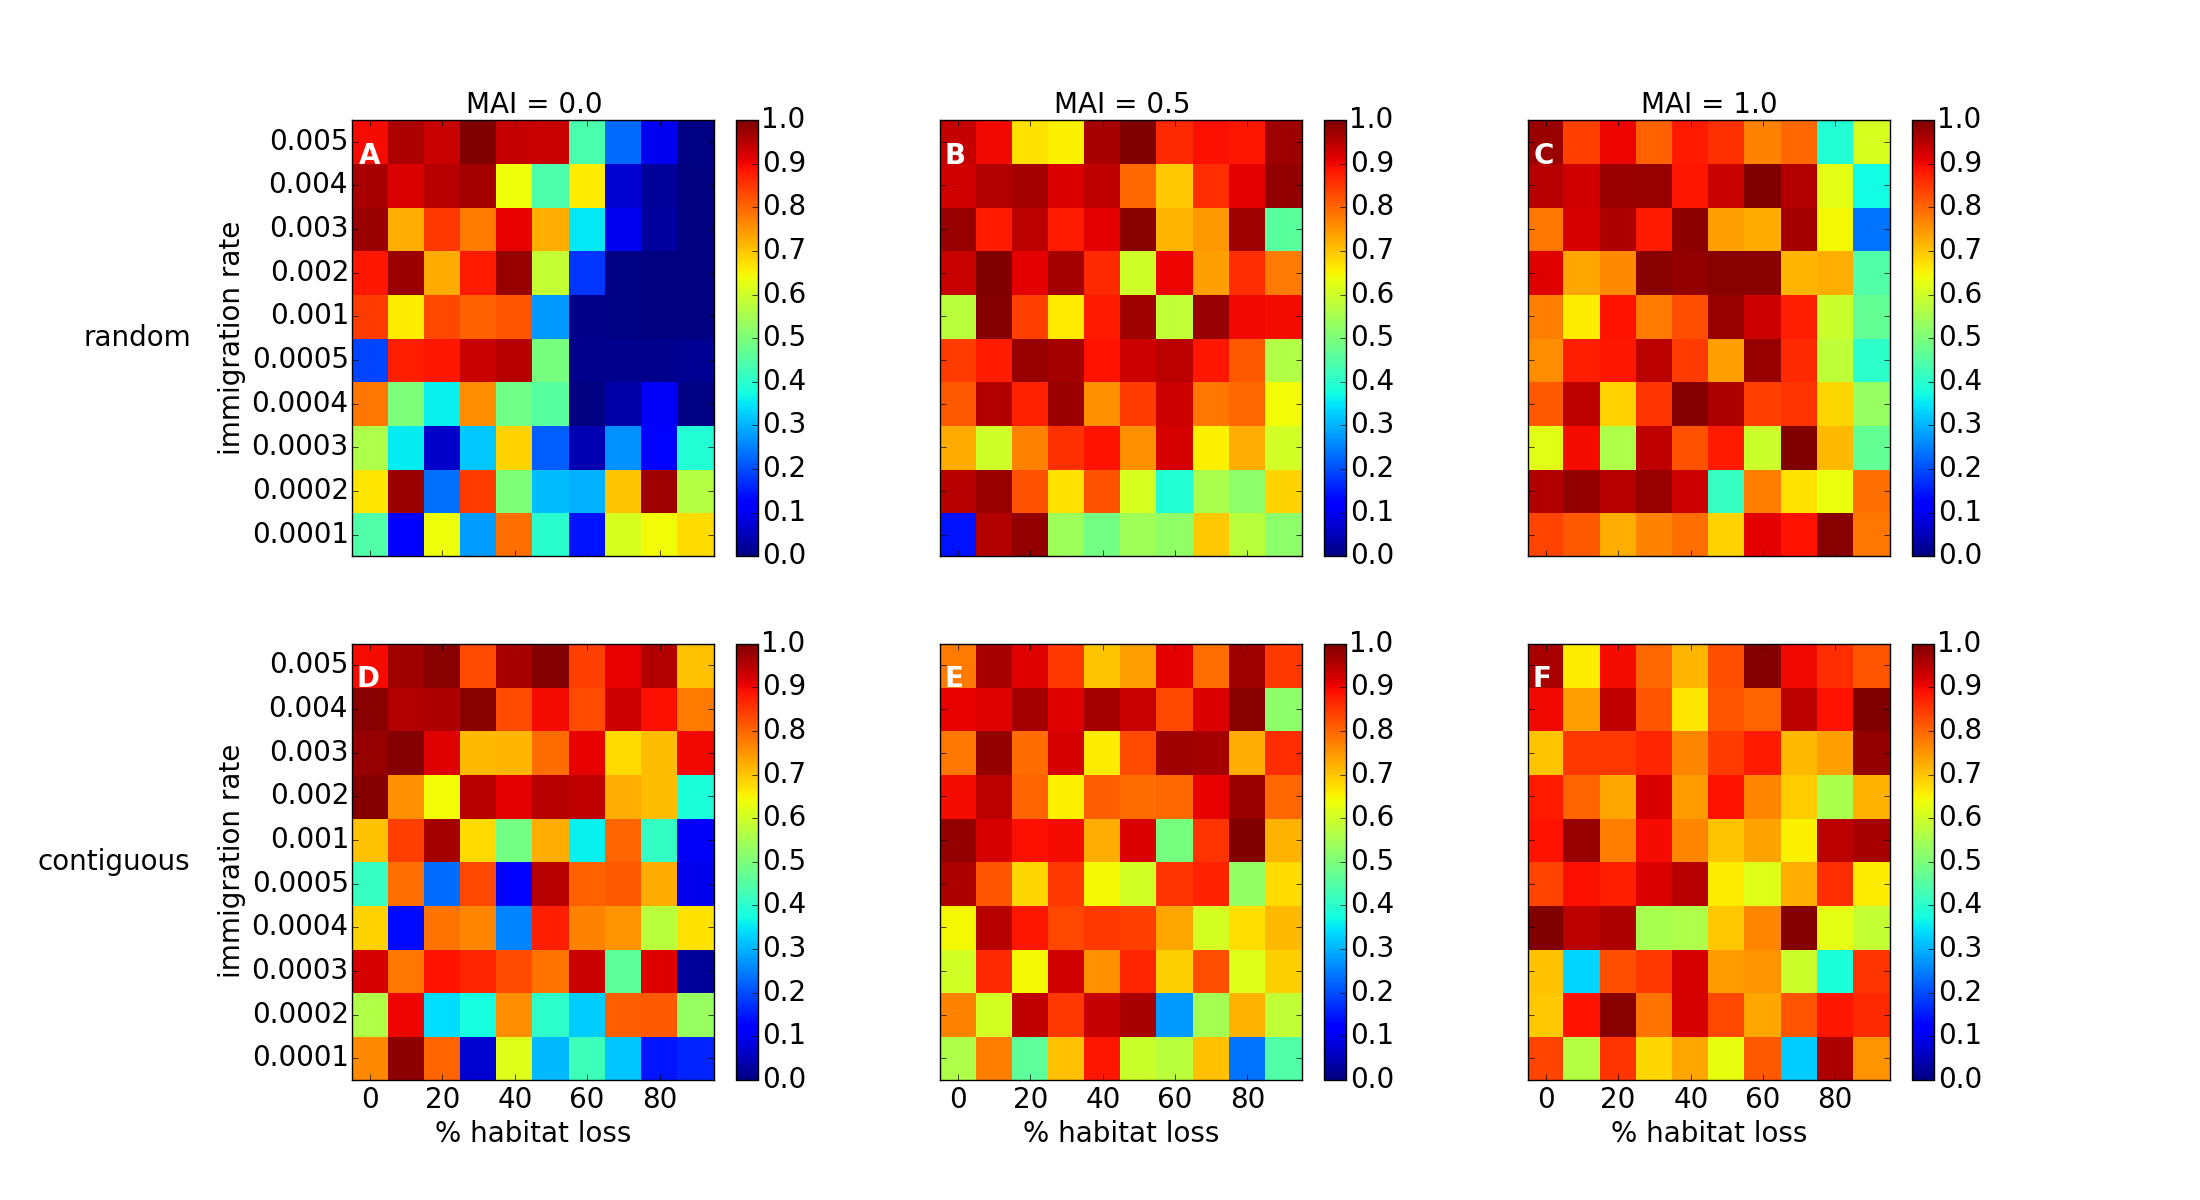
\includegraphics[width=\textwidth]{{{figures/clean_analysis/heatmap_ttest}}}
	\caption{P-values for t-tests to compare the \emph{Shannon equitability} calculated by two different sampling methods: \emph{snapshot} and \emph{averaged} sampling (see text for definitions). Each point in the plot represents the p-value of the test comparing the \emph{snapshot} and \emph{averaged} Shannon equitability results for the 50 replicate simulations at the corresponding HL and IR value. A p-value$<0.05$ (i.e.dark blue) represents $95\%$ confidence that the two sampling methods produce different average equitability results.}
	\label{fig:ttest}
\end{figure}

The \emph{Shannon equitability} metric (equation \eqref{eq:shan_eq}) is calculated for all simulations using two different sampling methods. The first method uses snapshot sampling (as in chapter \ref{chap:}) i.e. species abundances are measured on the last time step of the simulation. The second method takes the mean species abundance over the final 4000 time steps of the simulation. Results obtained using the two sampling methods are referred to as \emph{snapshot} and \emph{averaged}, correspondingly. We compare the results obtained using a \emph{two-sided t-test}, which is implemented in the \emph{Python} package \emph{scipy}. The test is used to compare two datasets of independent samples, testing the null hypothesis that the expected value of the two datasets are equal. If the \emph{p-value} of the test is smaller than the confidence threshold then there is sufficient evidence to reject the null hypothesis and conclude that the means of the two datasets are significantly different. For each test we are comparing the \emph{snapshot} and \emph{averaged} equitability results, calculated from the 50 replicate simulations at a given HL and IR value. If the test is significant then we conclude that the two sampling methods give significantly different results in calculation of the average Shannon equitability at that value of HL and IR. We conduct tests for all HL and IR values, and all three MAI ratios, under random and contiguous HL. The \emph{p-values} of these tests are depicted in figure \ref{fig:ttest}.  

In general figure \ref{fig:ttest} shows that there is strong support for the conclusion that the two sampling methods produce the same average equitability results. The worst case is random HL at MAI$=0.0$ (panel A). In this case there is a region of parameter space, above HL$=60\%$, where the p-values are significant. Therefore in this region the methods appear to give statistically different results. However, as stated, most of the tests suggest that the two methods produce statistically similar results. The similarity between the two methods is surprising given the results of the estimator analysis in section \ref{sec:convergence}. Presumably averaging over 50 replicate simulations provides some reduction in noise. It may also be that a high level of precision in the estimates of species abundances is not required to calculate community level metrics. Based on the comparison presented here we conclude that snapshot sampling is sufficient to draw general conclusions about community structure over the ensemble of simulations. This allows consistency with the analysis in chapter \ref{chap:habitat_loss_high_immigration}. However we acknowledge that the use of snapshot samples may introduce some error, and increased variability, into our calculations. We treat the region of parameter space in which the equitability results proved dissimilar (panel A: random HL. MAI$=0.0$) with particular caution.

NOTE: on network and diversity metrics - sample length of 200.

\subsection{Diversity}
\label{sec:vir_diversity}

\begin{figure}
	\includegraphics[width=\textwidth]{{{figures/clean_analysis/random/heatmap1}}}
	\caption{\textbf{Random HL:} Mean values of diversity metrics at each combination of HL and IR (Average over 50 replicate simulations). All metrics use snapshot sampling (see text). Each row corresponds to a different MAI ratio, as labelled. Panels A,D,G: Number of extinctions, defined as number of species with less than 3 individuals at end of simulation. Panels B,E,H: Total number of individuals in the community. Panels C,F,I: Shannon equitability metric.}
	\label{fig:vir_diversity_random_hp}
\end{figure}
%% These plotted with: files/habitat_loss_project/IBM/chapter5_analysis/random/plot_heatmap1.py
\begin{figure}
	\includegraphics[width=\textwidth]{{{figures/clean_analysis/contiguous/heatmap1}}}
	\caption{Similar to figure \ref{fig:vir_diversity_random_hp}, but for \textbf{contiguous HL}.}
	\label{fig:vir_diversity_contiguous_hp}
\end{figure}

Figures \ref{fig:vir_diversity_random_hp} and \ref{fig:vir_diversity_contiguous_hp} illustrate the mean value of three metrics over the region of parameter space, \emph{number of extinctions}, \emph{total number of individuals} and \emph{Shannon equitability}, for the random and contiguous scenarios respectively. All results shown are calculated from snapshot samples. As stated in section \ref{sec:exp_method}, an extinction is defined as the presence of less than three individuals in the landscape. The three metrics show broadly similar pattern across the region of parameter space in both HL scenarios. We highlight to following general observations:
\begin{itemize}
	\item Reducing IR increases the number of extinctions (panels A,D,G, both figures). In the contiguous case there are, on average, more extinctions than the random case. These extinction are clearly induced by habitat loss, appearing to increase monotonically along the HL gradient. Communities under random HL exhibit fewer extinctions. And, especially in mutualistic communities the number of extinctions appears to be less sensitive to HL.
	\item In antagonistic communities the total number of individuals varies with IR (panel B, both figures). Initially reducing IR reduces the number of individuals, but at the lowest IR values the number of individuals increases again. In mutualistic communities the dependence of total individuals on IR is greatly reduced, if not removed altogether (panels E,H, both figures). In all cases HL reduces the number of individuals, as expected and in agreement with the results from chapter \ref{chap:habitat_loss_high_immigration}.
	\item In general mutualistic communities have higher total abundance than antagonistic ones. Under contiguous HL they exhibit more extinctions.
	\item In all cases reducing the IR reduces the Shannon equitability i.e. communities become less even. On the whole communities become more even under random HL (panels C,F,I, figure \ref{fig:vir_diversity_random_hp}), as observed in chapter \ref{chap:habitat_loss_high_immigration}. However at some IRs random HL appears to make antagonistic communities more even (IR$=0.0003$ to $0.002$, panel C, figure \ref{fig:vir_diversity_random_hp}). Also in the contiguous scenario, at certain IRs, antagonistic communities become less even along the HL gradient (IR$=0.0002$ to $0.003$, panel C, figure \ref{fig:vir_diversity_contiguous_hp}). This effect is not clear in the case of mutualistic communities, where there is little visible dependence of equitability on HL (panels F,I figures \ref{fig:vir_diversity_random_hp}).
\end{itemize}

The observations listed above confirm some of our predictions from section \ref{sec:motivate_immigration}. The role of immigration in driving evenness is clear, since reducing IR reduces the Shannon equitability in all cases. In the random scenario there is some evidence that lower IRs reduces the magnitude of the change in evenness, as predicted. And in both scenarios there appear to be some cases where the evenness of the communities decrease with HL. This requires further analysis. Also the predicted extinctions are observed at low IR, due to a smaller \emph{rescue effect}. However in the random scenario the number of extinctions does appear very sensitive sensitive to HL, which is unexpected. This, and the fact that the random scenario produces fewer extinctions than the contiguous, suggest that the mechanisms behind the species extinctions differ between the two scenarios. Based on what we saw in chapter \ref{chap:habitat_loss_high_immigration} we propose that extinctions in the contiguous scenario are due to strong predation driven by high IS, whereas in the random scenario they are likely due to a collapse in the trophic structure of the community due to low IS.

The diversity results also highlight certain other new and unexpected features. In particular we find that MAI ratio play an important role in mediating how communities respond to HL across the range of IR values. This role is most clearly visible in the total number of individuals, which becomes insensitive to IR at high MAI ratios. In this sense at least mutualism can be said to confer robustness on communities in the face of variable IR. However, based on the persistence analysis in section \ref{sec:mvp}, we may expect that the mutualistic communities at low IR are dominated by a small number of species in the non-basal trophic levels. It is perhaps the increased dominance of these species which accounts for the constant total abundance across the range of IR values. From the equitability results we know that, although abundance may not change, mutualistic communities do become less even at low IR. It will be informative to study community composition in more detail for such cases.


\subsection{Variability and interaction strengths}
\label{sec:vir_variability}

\begin{figure}
	\includegraphics[width=\textwidth]{{{figures/clean_analysis/random/heatmap3}}}
	\caption{Similar to figure \ref{fig:vir_diversity_random_hp}, but showing three different metrics: the natural logarithm of the mean interaction strength (ln(mean IS)); the total number of interactions between all species; and the natural logarithm of the mean temporal variability (ln(mean CV)). \textbf{Random HL}.}
	\label{fig:vir_var_random}
\end{figure}
%% These plotted with: files/habitat_loss_project/IBM/chapter5_analysis/random/clean_plot_hm3.py
\begin{figure}
	\includegraphics[width=\textwidth]{{{figures/clean_analysis/contiguous/heatmap3}}}
	\caption{Similar to figure \ref{fig:vir_var_random}, but for \textbf{contiguous HL}.}
	\label{fig:vir_var_contiguous}
\end{figure}

Figures \ref{fig:vir_var_random} and \ref{fig:vir_var_contiguous} show the mean value of three variability and interaction strength metrics for the random and contiguous scenarios respectively. Panels A,D, and G show the natural-logarithm of the mean interaction strength (IS, defined in section \ref{:sec:def_iss}). Panels B,E, and H show the total number of (inter-specific) interaction events between all individuals, and the remaining panels show the natural-logarithm of the temporal variability metric (mean CV) (defined in section \ref{sec:def_stability_metrics}). The results for the contiguous scenario are simplest (figure \ref{fig:vir_var_random}), and are summarised as follows:
\begin{itemize}
	\item Interaction strength and temporal variability increase with contiguous HL in all cases. So varying IR does not change the response of these metrics that was observed in chapter \ref{chap:habitat_loss_high_immigration}.
	\item Reducing IR increases temporal variability, as predicted. The increase in variability is associated with a slight increase in interaction strengths, which is weaker at high MAI.
	\item For antagonistic communities the number of interactions decreases with both IR and HL. For mutualistic communities the the number of interactions decreases with HL, but is less sensitive to IR.
\end{itemize}

In the random scenario there is a more subtle interaction between HL and IR. We observe the following from figure \ref{fig:vir_var_contiguous}:
\begin{itemize}
	\item The response of the total number of interactions is qualitatively the same as in the contiguous case. However slightly more interactions are lost due to random HL than contiguous HL, in agreement with the results from chapter \ref{chap:habitat_loss_high_immigration}
	\item As in the contiguous case, reducing IR increases variability, with an associated increase in IS. However, especially at intermediate IR values, increasing HL initially reduces variability but causes variability to increase at high levels of destruction. Visually the profile of changing variability along the HL gradient appears to be approximately but not exactly correlated with changes in IS.   
\end{itemize}

The results can largely be extrapolated form those in the previous two chapters and confirm our predictions. There are no surprises in the contiguous case. Although we note the variability and IS responses are consistent with, and therefore support conclusions drawn from, previous analysis. Also the similarity between the results for number of interactions and number of individuals, in both HL scenarios, supports our assertion from chapter \ref{chap:habitat_loss_high_immigration} that interaction frequencies are largely driven by abundance. We did not expect to see an increase in IS as IR is reduced, an effect which is present in all cases. However we did predict that effects due to species interaction would come to play a more important role as immigration was reduced. It is not clear why reducing IR increases the mean probability of trophic interactions between species (see discussion in section \ref{sec:res_synthesis} for interpretation of IS in terms of probability). We suggest that it may be due to the dominance of communities by abundant and strongly interacting species. This hypothesis is investigated in section \ref{sec:WHERE}. 

The variability response under random HL is another unexpected feature. In many instances random HL causes an initial decline, followed by a subsequent increase in temporal variability. This pattern appears robust across IRs and MAI ratios (panels C,F,I, figure \ref{fig:vir_var_random}). In fact, returning to figure \ref{fig:strong_fig} the same effect is present in our original results. The temporal variability increases at $90\%$ HL. We explore this feature further in section \ref{sec:whereis} below.

\begin{figure}
	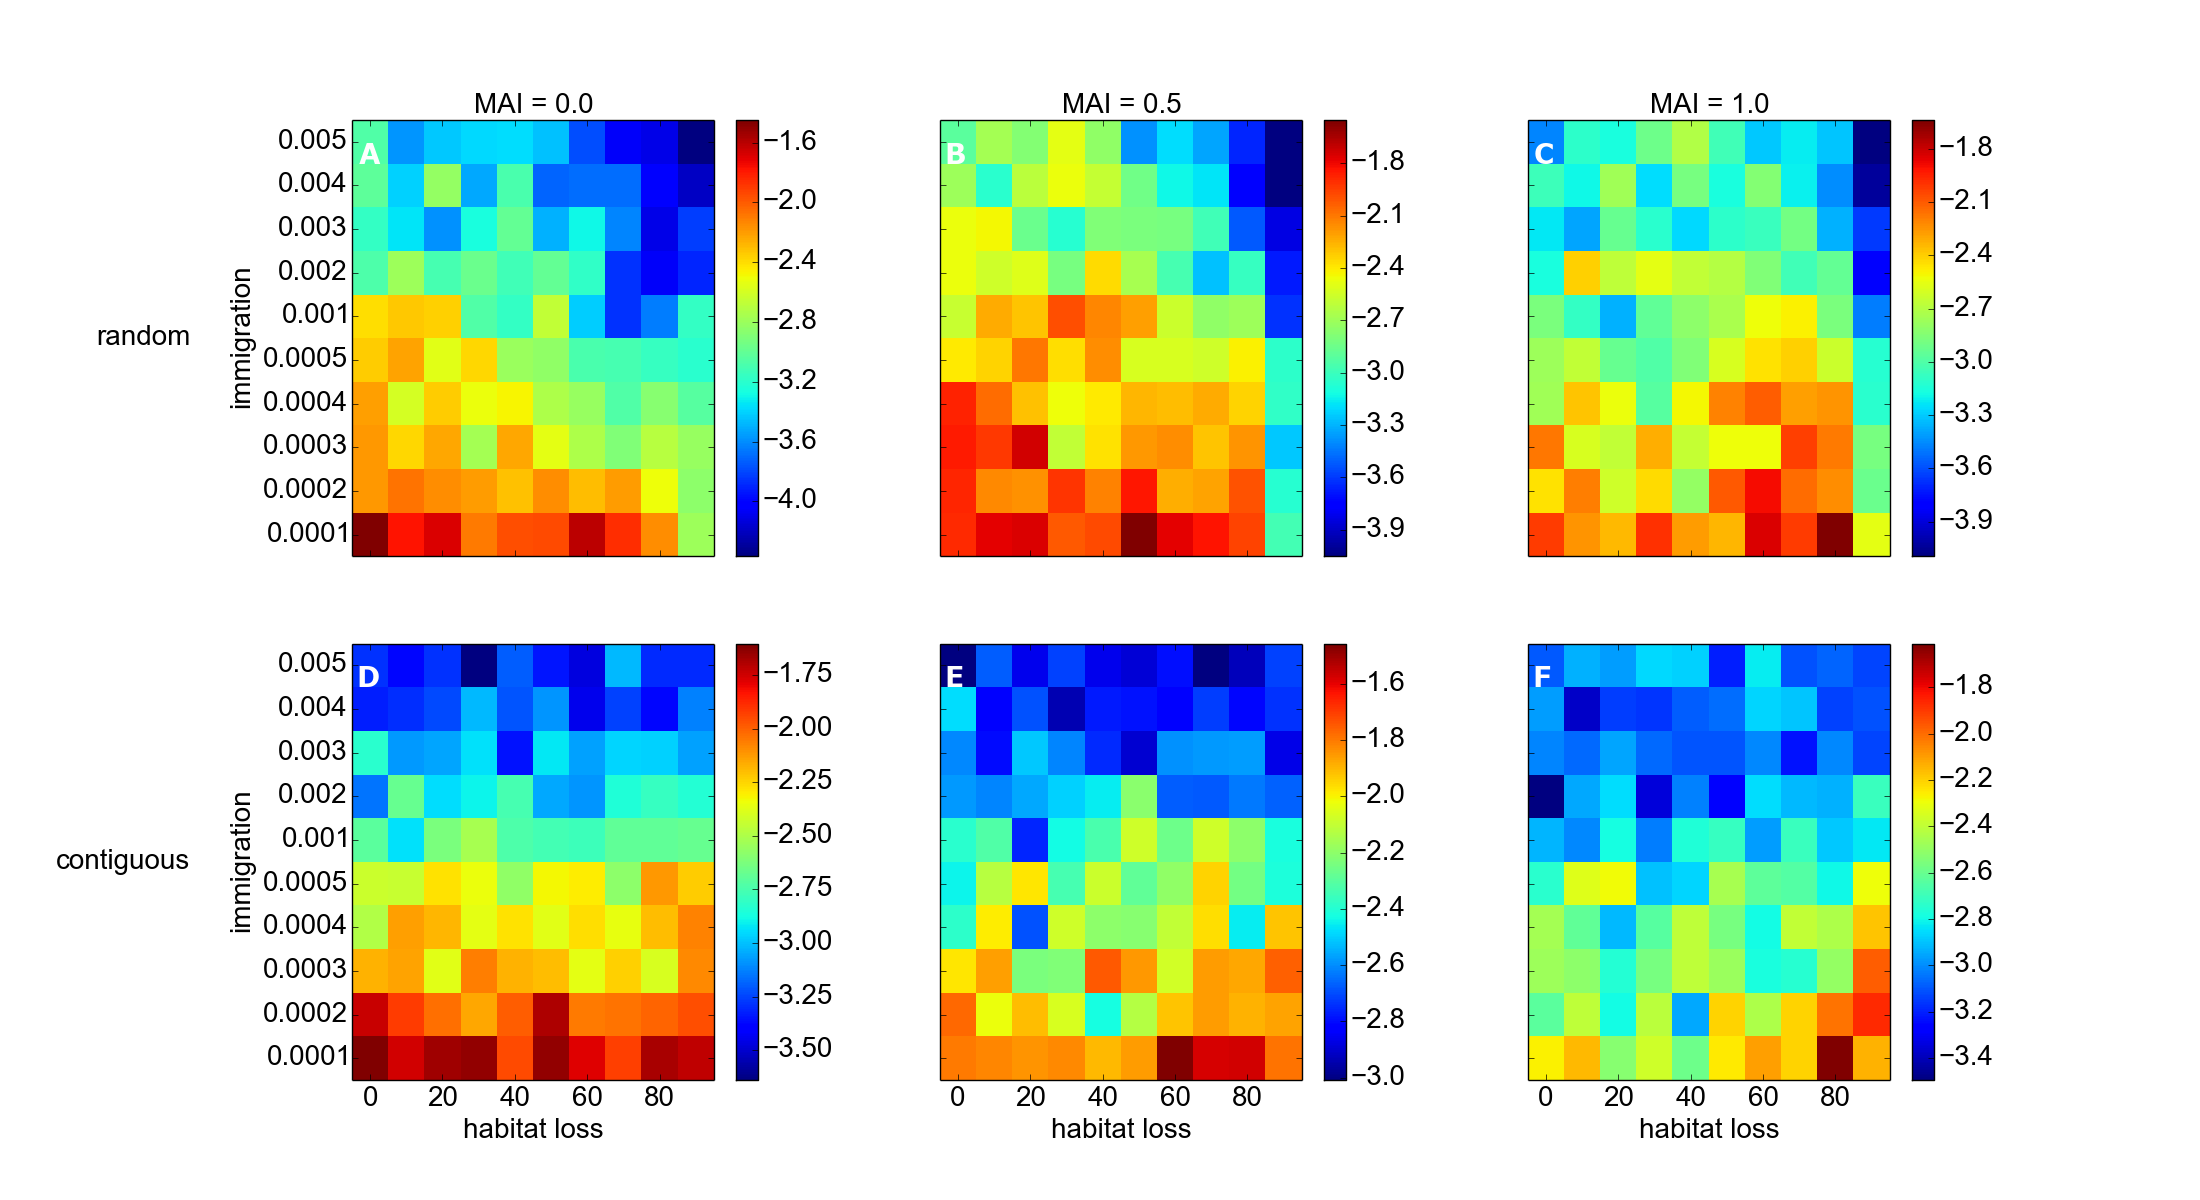
\includegraphics[width=\textwidth]{{{figures/clean_analysis/heatmap_sync}}}
	\caption{Natural logarithm of \emph{ecosystem synchrony} (ln($Sync$), defined in section \ref{sec:def_invariability} for both HL scenarios, and all three MAI ratios.}
	\label{fig:vir_sync_hm}
\end{figure}


%% Don't necessarliy want to analyse invariability metrics:
%\begin{figure}[hb]
%	\includegraphics[width=\textwidth]{{{figures/clean_analysis/random/heatmap_inv}}}
%	\caption{Random HL. Ecosystem synchrony. Ecosystem invariability. Population invariability.}
%\end{figure}
%
%\begin{figure}[hb]
%	\includegraphics[width=\textwidth]{{{figures/clean_analysis/contiguous/heatmap_inv}}}
%	\caption{Contiguous HL. Ecosystem synchrony. Ecosystem invariability. Population invariability.}
%\end{figure}


\subsection{Dependence on immigration}
\label{sec:dependence_on_im}

%% This figure produce by: /MyFiles/cm1788/Documents/IM_vs_HL_heatmap/clean_results/random/plot_immap.py
%% Might need to re-scale if colours not clear when printed?
\begin{figure}[hb]
	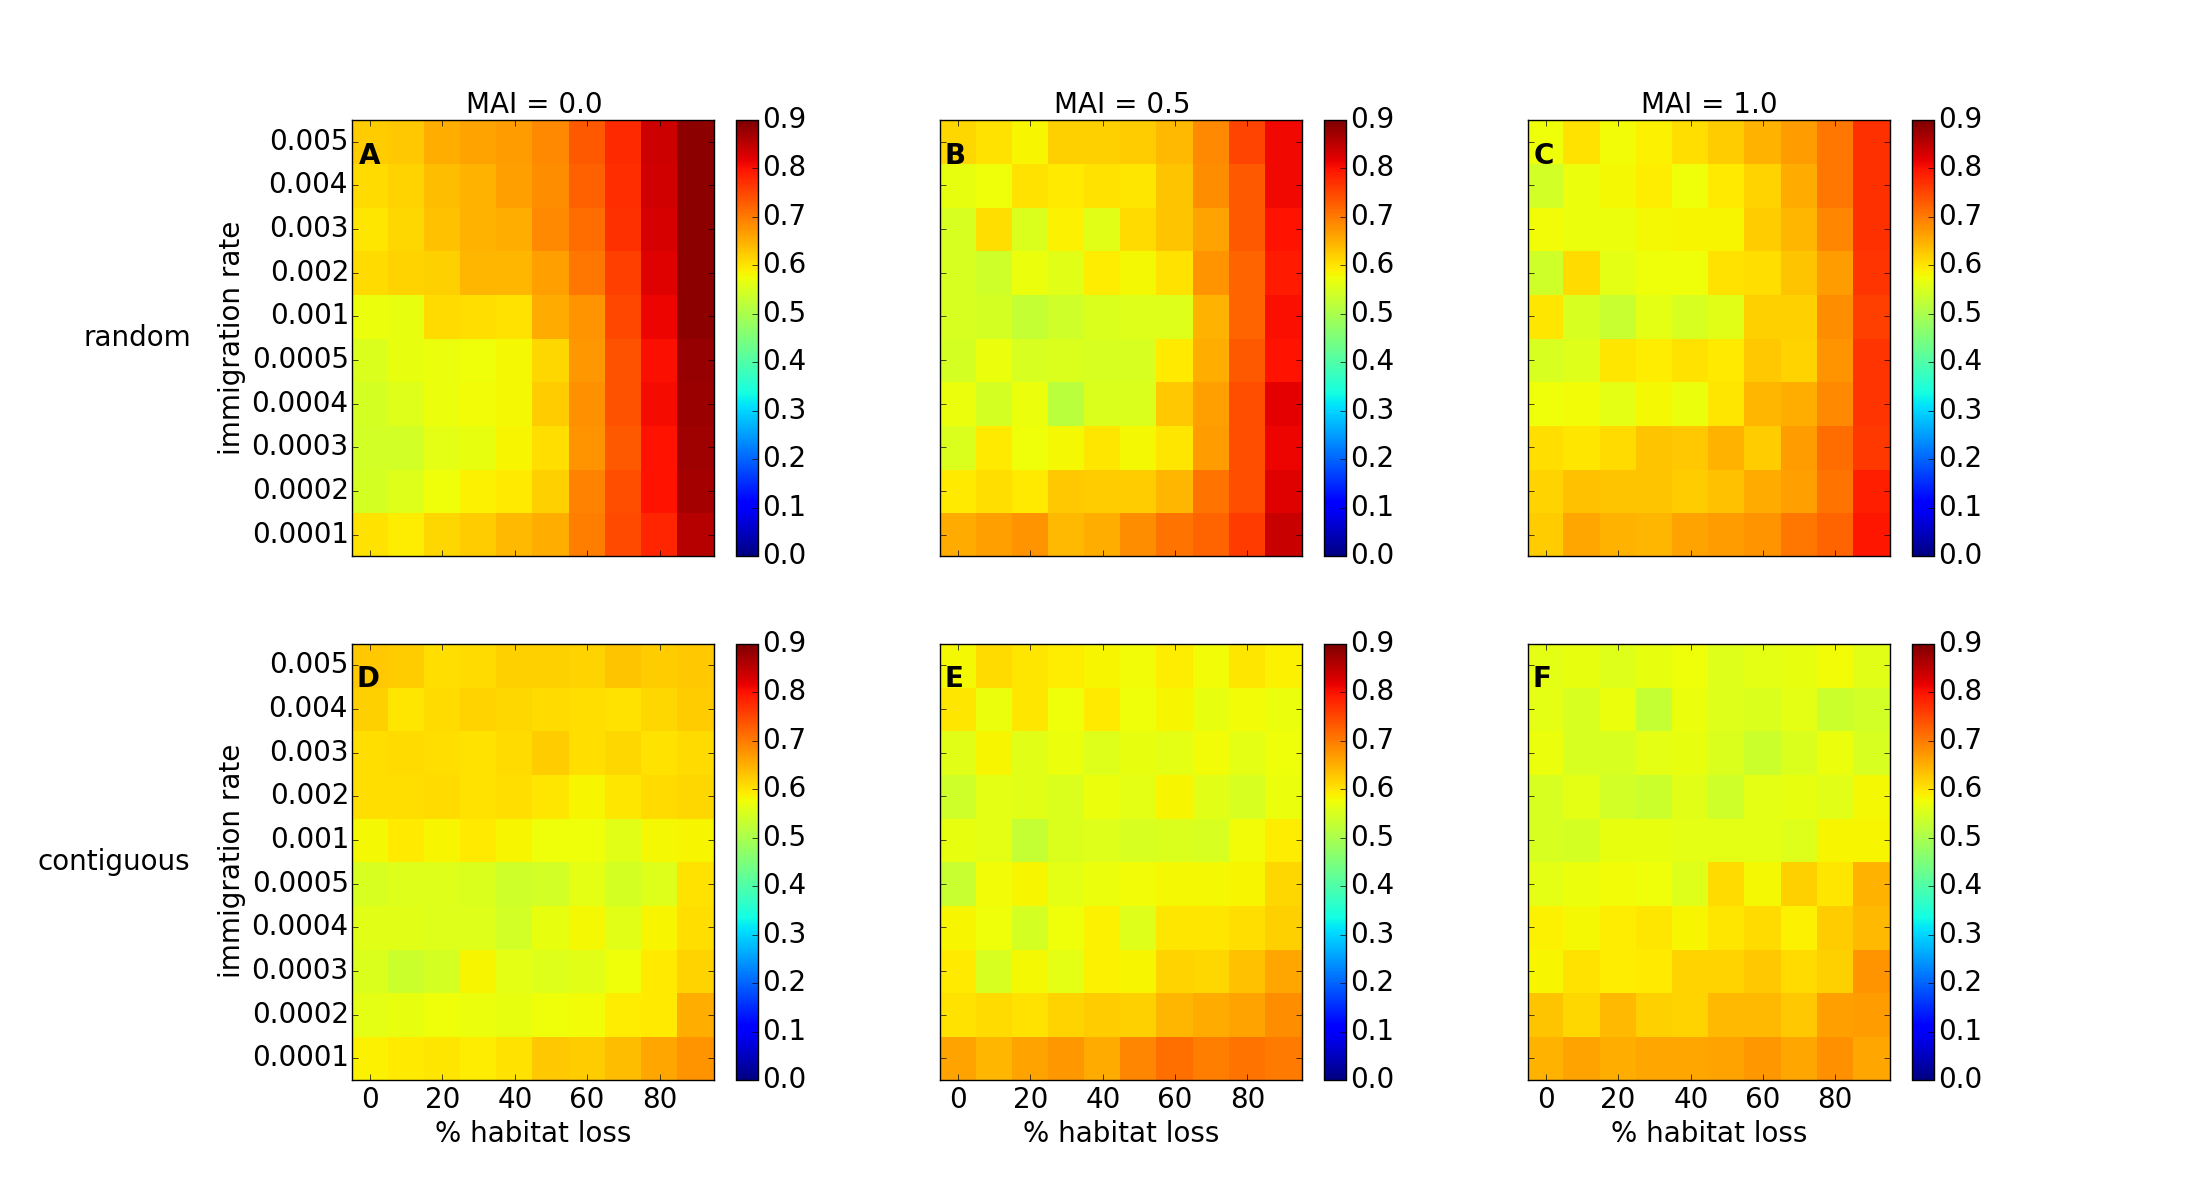
\includegraphics[width=\textwidth]{{{figures/clean_analysis/heatmap_proportion_im}}}
	\caption{Similar to figure \ref{fig:vir_sync_hm}, but displaying the proportion of the total number of individuals born that come from immigration, calculated as in figure \ref{fig:res_proportion_immigrants}.}
	\label{fig:proportion_im_heatmap}
\end{figure}


\section{Bivariate analysis: fixed IR}
\label{sec:biv_fixIR}
In this section we will present results for a fixed, low IR value against HL. And for a fixed intermediate HL value against IR.

\begin{itemize}
	\item Differential response of mutualistic and antagonistic communities - needs investigating. Community composition, esp MAI ratios under changing IR.
	\item Do communities really become less even at some IRs (bivariate analysis), and is this associated by a reduced dependence on immigration...
	\item Why does abundance suddenly increase at low IR in antagonistic communities?
	\item Why does contiguous HL generate more extinctions? And why are extinctions not dependent on HL in the random case?
	\item Why does IS increase as IR reduced? Dominant species? Check distribtuions..
	\item What is going on with variability in the random scenario? (Does new metric meancv\_sqaured solve it?)
	
	\item Proportion of immigration not as as simple as expected..
\end{itemize}

In this section we look in more detail at the results summarised in section \ref{sec:init_res} by conducting bivariate analysis of certain key metrics\footnote{Which ones. Also this section, and the following one?}, as we did in chapter \ref{chap:habitat_loss_high_immigration}. From the depiction of how metrics vary across the slice of parameter space we select an immigration rate (IR) of $0.0005$ at which to study the response of communities to HL. The IR is an order of magnitude below the \emph{default value} of $0.005$ used in chapter \ref{chap:habitat_loss_high_immigration}. The choice of such an IR here is justified by..

\subsection{Evenness}
\label{sec:biv_HL_evenness}

In chapter \ref{chap:hhl} we saw that species abundances became more even under random HL, while they evenness did not change significantly under contiguous HL. These changes we attributed to the dependence of communities on immigration, which acts to make the distribution of individuals across species more even. Therefore we expected that at low IR we may observe a change in the evenness response. The IR of $0.0005$ was chosen because it appeared to generate communities that became less even under contiguous HL, especially in the case of MAI$=0.0$.

From figure \ref{fig:biv_HL_proportion_im} we see that the dependence on immigration is lower across the HL gradient than was observed when using the default IR. This can 

Figure \ref{fig:biv_HL_shannon_eq} shows how the \emph{Shannon equitability} metric, calculated at the community level, changes across the HL gradient under both HL scenarios. This metric (equation \eqref{eq:shan_eq}) measures how evenly abundance is distributed between all species in the community. From the figure we see the characteristic feature that low MAI communities are more even than high MAI communities (chapter \ref{chap:} and \cite{lurgi2015effects}). We also observe that under both types of HL antagonistic communities (MAI$=0.0$) \emph{become less even}. This is a new observation, which we seek to explain below\footnote{HOw?}. Communities with mixed interactions between the first two trophic levels (MAI$=0.5$) do not become significantly more or less even under either type of HL, while mutualistic communities (MAI$=1.0$) respond in opposite directions. Mutualistic communities become more even and less even under random and contiguous HL respectively. The observation that varying the level of mutualism causes communities to respond differently to HL is a new and interesting feature of these results. 

We explore the evenness response further by calculating the Shannon equitability within each trophic level. These results are shown in figure \ref{fig:biv_HL_shannon_eq_TL}. These plots reveal that there is a difference between the  equitability response at the community level compared to the that within trophic levels, especially under random HL. In the random scenario (panels A,C,E,G) the distribution of abundances within all trophic levels become more even, except for the top trophic level of the antagonistic communities (panel G). In the contiguous scenario antagonistic communities  become less even within trophic levels, whereas mutualistic communities (MAI$=0.5,1.0$) do not exhibit changes in evenness within trophic levels.   

\begin{figure}
	\centering	
	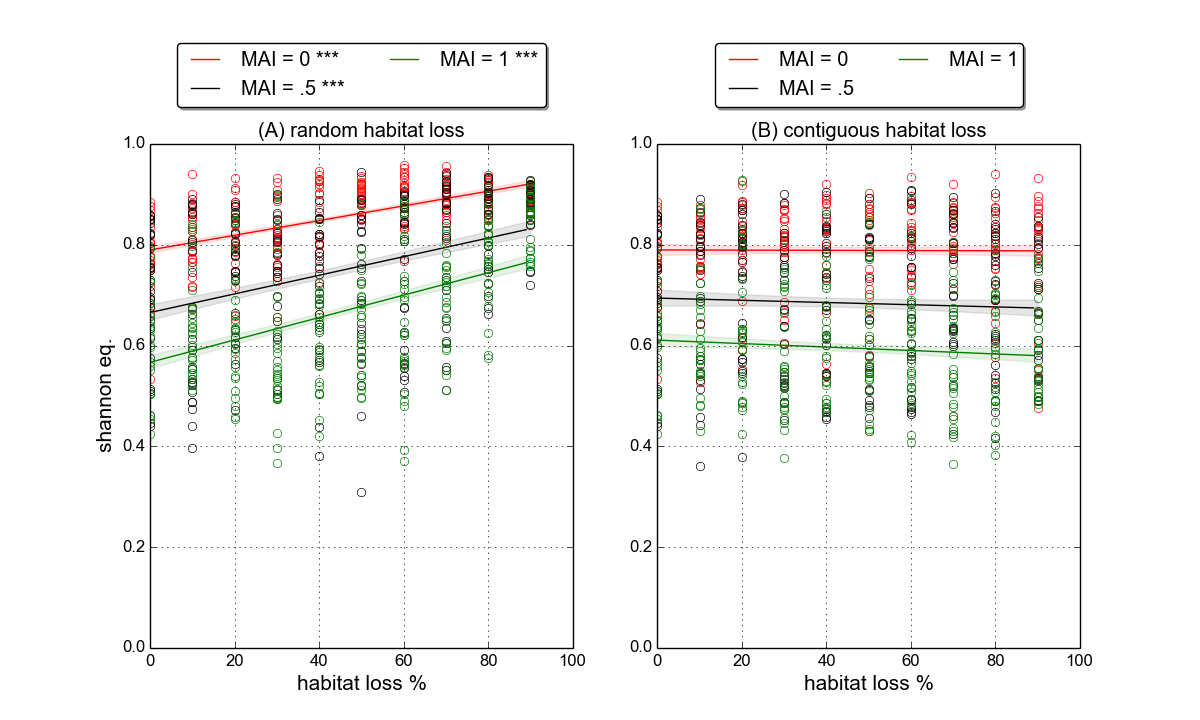
\includegraphics[width=\textwidth]{{{figures/bivariate_v_HL/clean_lm_shannon_eq_3mai}}}
	\caption{\textbf{Shannon equitability} against percentage habitat loss, for both scenarios: (A) Random HL, and (B) Contiguous HL. Circles represent the Shannon index value for a single community; lines represent a linear fit to the data and the shaded regions indicate the standard error of the mean Linear fits and p-value markers as in previous plots (see caption of figure \ref{fig:WHEREFIRST}).}
	\label{fig:biv_HL_shannon_eq}
\end{figure}

\begin{figure}
	\centering	
	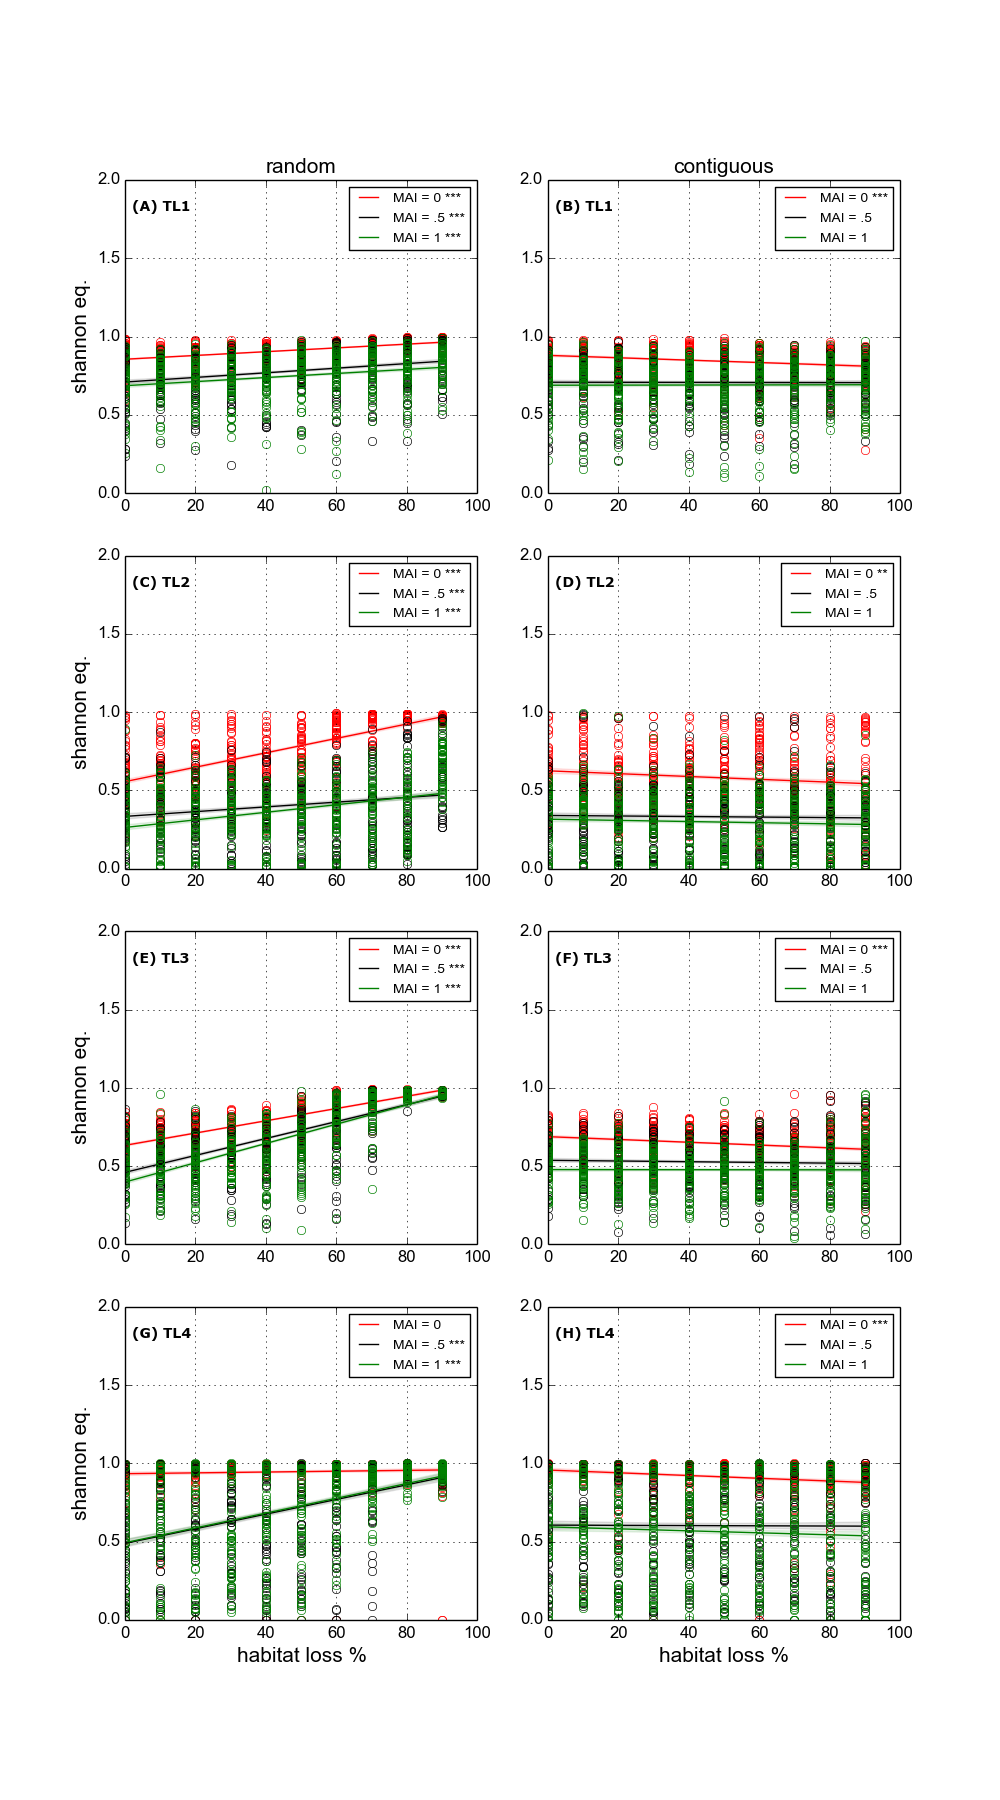
\includegraphics[width=0.7\textwidth]{{{figures/bivariate_v_HL/lm_fg_shannon_eq_hl_contiguous_3mai}}}
	\caption{\textbf{Shannon equitability} against percentage habitat loss, for each trophic level. Left column: random HL. Right column: contiguous HL. Circles represent the Shannon index value for a single community; lines represent a linear fit to the data and the shaded regions indicate the standard error of the mean. Linear fits and p-value markers as in previous plots (see caption of figure \ref{fig:WHEREFIRST}).}
	\label{fig:biv_HL_shannon_eq_TL}
\end{figure}

The above changes in evenness can be understood by looking at example rank-abundance distributions (RADs - section \ref{sec:define_rads}) for single communities at different levels of HL. Figure \ref{fig:biv_HL_rads_mai0_random} shows the RADs for three antagonistic communities (MAI$=0.0$) under random HL. Firstly the discontinuity in the distribution at HL$=90\%$ makes the interpretation of the model fits problematic. Therefore we use only the Shannon metric in the current analysis:
\begin{itemize}
	\item Being an antagonistic community, the RAD at HL$=0\%$ is quite even.
	\item  At the community level the distribution becomes less even due to HL. The RAD at HL$=90\%$ is dominated by 16 plant species, with all other species having a relative abundance of less than 0.01.
	\item  However within trophic levels, as indicated by the colours, the increase in evenness is visually clear (except for the top trophic level). This is especially visible for the plant communities.
\end{itemize}

%% Not sure about this plot: interesting, but may confuse the message, just see example RADs
%\begin{figure}
%	\centering	
%	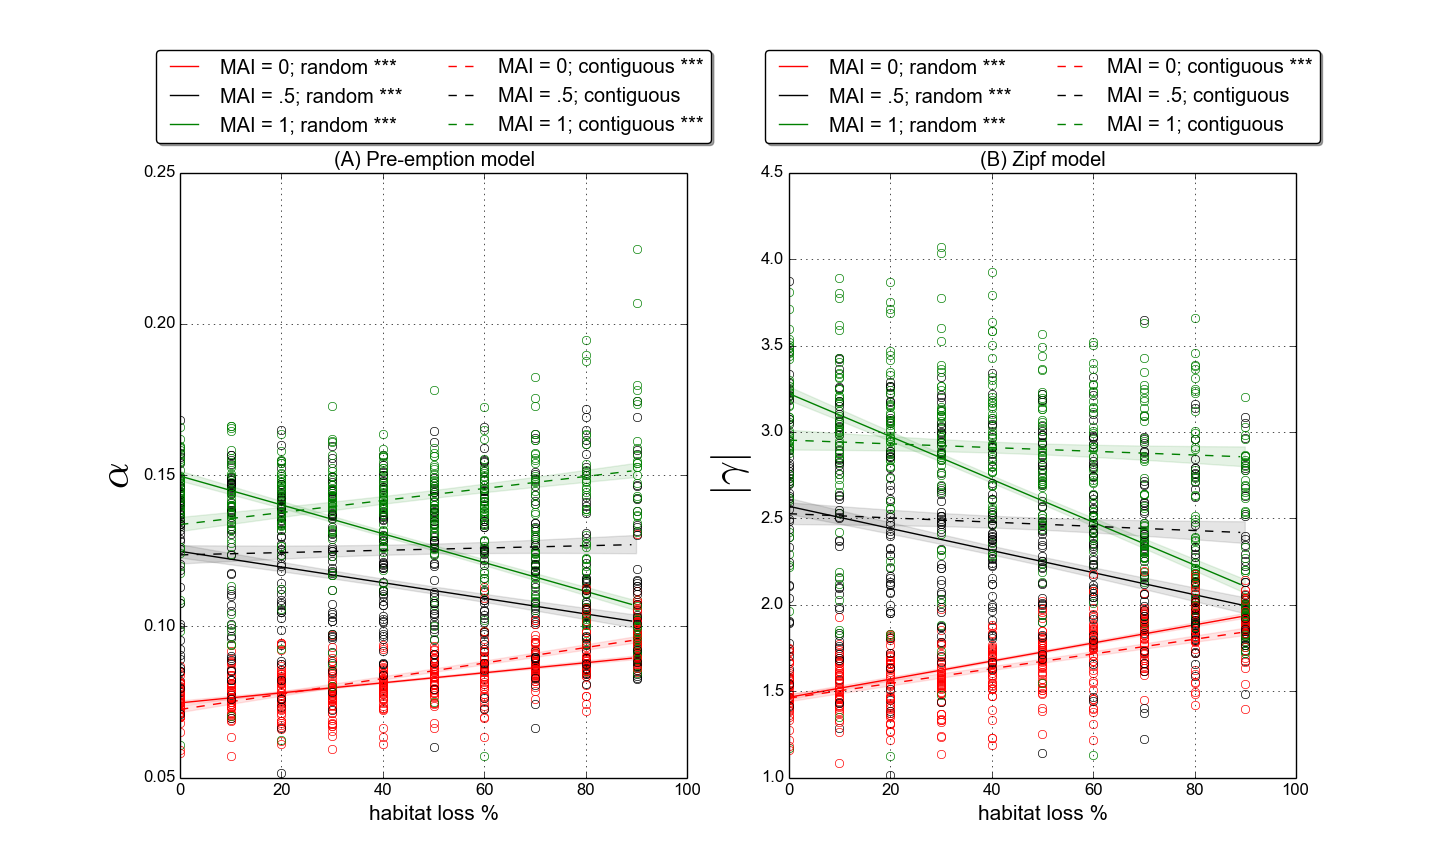
\includegraphics[width=\textwidth]{{{figures/bivariate_v_HL/lm_radfit_params_v_hl}}}
%	\caption{\textbf{Rank abundance model fit} parameters against HL. Panel A: Pre-emption model parameter $\alpha$ is smaller for more even distributions. Panel B: Absolute value of Zipf model parameter $\left| \gamma \right|$ is smaller for more even distributions. (See model definitions in section \ref{sec:define_rads}). Solid lines represent linear fits to the random HL data, dashed lines indicate linear fits to the contiguous HL data, and error bars give $\pm 1$ standard-deviation. *** indicates p-value $<0.001$ for linear model fit, whilst no marker indicates p-value$>0.1$.}
%	\label{fig:biv_HL_radfit}
%\end{figure}


\begin{figure}
	\centering	
	\includegraphics[width=\textwidth]{{{figures/bivariate_v_HL/example_RADS_mai0_random}}}
	\caption{\textbf{Example RADs} MAI 0. Random}
	\label{fig:biv_HL_rads_mai0_random}
\end{figure}

Figure \ref{fig:biv_HL_rads_mai1_random} shows RADs for mutualistic communities (MAI$=1.0$) under random HL:
\begin{itemize}
	\item Mutualistic, therefore less even in pristine habitat. In fact dominated by 10 abundant species, as seen at zero IR (chapter \ref{chap:stress_testing}).
	\item RAD flattens out due to HL - becoming more even at community level, and within trophic levels. Although there is still a discontinuity at HL$=90\%$. 
	\item Species in this tail sustained only by immigration? But not subject to predation pressure and therefore not driven to extinction?
\end{itemize}

\begin{figure}
	\centering	
	\includegraphics[width=\textwidth]{{{figures/bivariate_v_HL/example_RADS_mai1_random}}}
	\caption{\textbf{Example RADs} MAI 1. Random}
	\label{fig:biv_HL_rads_mai1_random}
\end{figure}

Figure \ref{fig:biv_HL_rads_mai0_contiguous} shows RADs for antagonistic communities (MAI$=0.0$) under contiguous HL:
\begin{itemize}
	\item Relatively even in pristine landscape, like figure \ref{fig:biv_HL_rads_mai0_random}.
	\item Becomes slightly less even at community and trophic levels. 
	\item However the discontinuity characteristic of the random scenario is not present. Presumably in the contiguous case these rare species are still able to interact, therefore reproduce and feed, and are fed upon.
\end{itemize}

\begin{figure}
	\centering	
	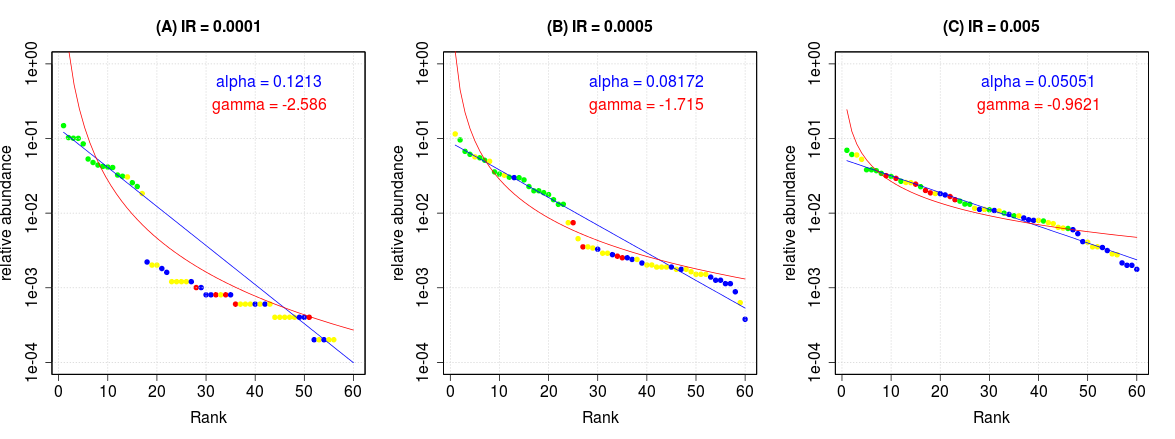
\includegraphics[width=\textwidth]{{{figures/bivariate_v_HL/example_RADS_mai0_contiguous}}}
	\caption{\textbf{Example RADs} MAI 0. Contiguous}
	\label{fig:biv_HL_rads_mai0_contiguous}
\end{figure}

Figure \ref{fig:biv_HL_rads_mai1_contiguous} shows RADs for mutualistic communities (MAI$=1.0$) under contiguous HL:
\begin{itemize}
	\item Less even in pristine landscape, although discontinuity not extreme in this community.
	\item Becomes slightly less even at community and trophic levels. 
	\item No clear change in evenness due to HL.
	\item Again do distinct `tail' of low abundance species, as in the random scenario.
\end{itemize}

\begin{figure}
	\centering	
	\includegraphics[width=\textwidth]{{{figures/bivariate_v_HL/example_RADS_mai1_contiguous}}}
	\caption{\textbf{Example RADs} MAI 1. Contiguous}
	\label{fig:biv_HL_rads_mai1_contiguous}
\end{figure}

Figure \ref{fig:biv_HL_proportion_im} shows the mean dependence on immigration:
\begin{itemize}
	\item In both cases dependence on immigration is lower than in chapter \ref{chap:}, which makes sense since the IR is lower.
	\item In the random scenario HL increases dependence on immigration for all MAI ratios. As in first chapter.
	\item This explains the increase in evenness within trophic levels, and the community level response of the antagonistic communities. However it does not explain the community level decrease in evenness of antagonistic communities  - this must be due to differences between trophic levels (or functional groups). For example plants become much more abundant relative to other groups. (See relative abundance plots below). 
	\item In the contiguous scenario there is a very slight increase in dependence on immigration. 
	\item Therefore we cannot explain the decrease in evenness under contiguous HL, which is especially pronounced for antagonistic communities. It is also clear the dependence on immigration \emph{is not to only determinant of evenness}.\footnote{The converse is that dependence in interactions reduces evenness? Also we know that mutualism reduces evenness..but these communities don't get less even. They are less even to start off with.}  
\end{itemize}

\begin{figure}
	\centering	
	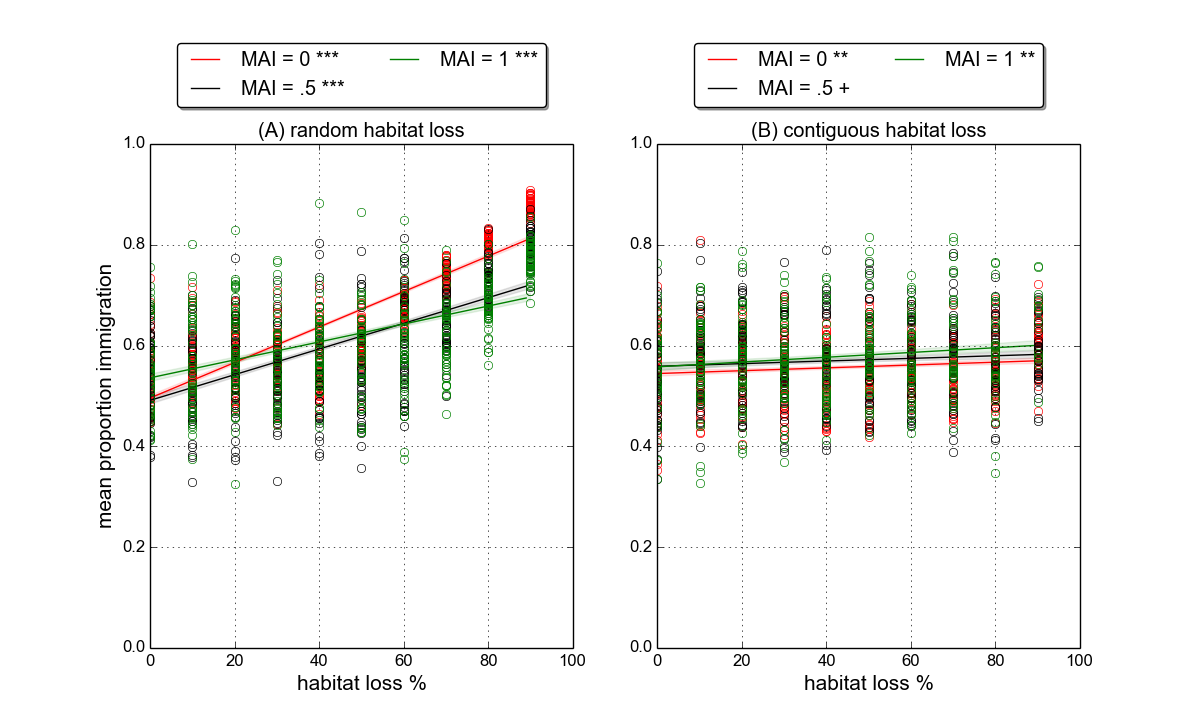
\includegraphics[width=\textwidth]{{{figures/bivariate_v_HL/lm_mean_proportion_immigration_3mai}}}
	\caption{\textbf{Number of immigrants} as a fraction of the total number of new individuals created over the course of a simulation. Linear fits and p-value markers as in previous plots (see caption of figure \ref{fig:WHEREFIRST}).}
	\label{fig:biv_HL_proportion_im}
\end{figure}

Figure \ref{fig:biv_HL_proportion_by_fg_random} shows the relative abundance of each functional group under random HL:
\begin{itemize}
	\item Top predator much lower in abundance than with default IR, even in pristine landscape. Partly due to removal of feeding links. Also due to lower IR - less food available, hits this group hardest?
	\item Basal species benefit, relatively, from random HL - reduced predation pressure
	\item All other functional groups suffer - same reasoning given in first chapter: less feeding, less mating.
	\item Plant come to dominate antagonistic communities at more than 0.9 RA. This explains the loss of evenness at the community level - it is due to the differential response of plant and other FGs.
	\item In mutualistic communities, although plant abundance increase relative to other groups they do not totally dominate - combined both types of plant is about 0.7 at MAI=$1.0$. This is because mutualistic animals retain their abundance quite well - about 0.3 and MAI$=1.0$. This partly explains why evenness response is different in mutualistic communities.
	\item Although RAs fall very low under random HL, this does not translate into extinctions,as we saw.
\end{itemize}

Figure \ref{fig:biv_HL_proportion_by_fg_contiguous} shows the relative abundance of each functional group under contiguous HL:
\begin{itemize}
	\item Slight decrease in both predator groups. Realistic. But why, when trophic interaction remain strong?
	\item Increase in non-mutualistic plants - reduced predation??
	\item Increase in mutualistic animals at MAI$=1.0$ - reduced predation while plant resource remains strong. But why no benefit other groups?
	\item Otherwise first two trophic level pretty constant (as in first chapter)
	\item These patterns hard to explain. Also relate to extinctions??
\end{itemize}
\begin{figure}
	\centering	
	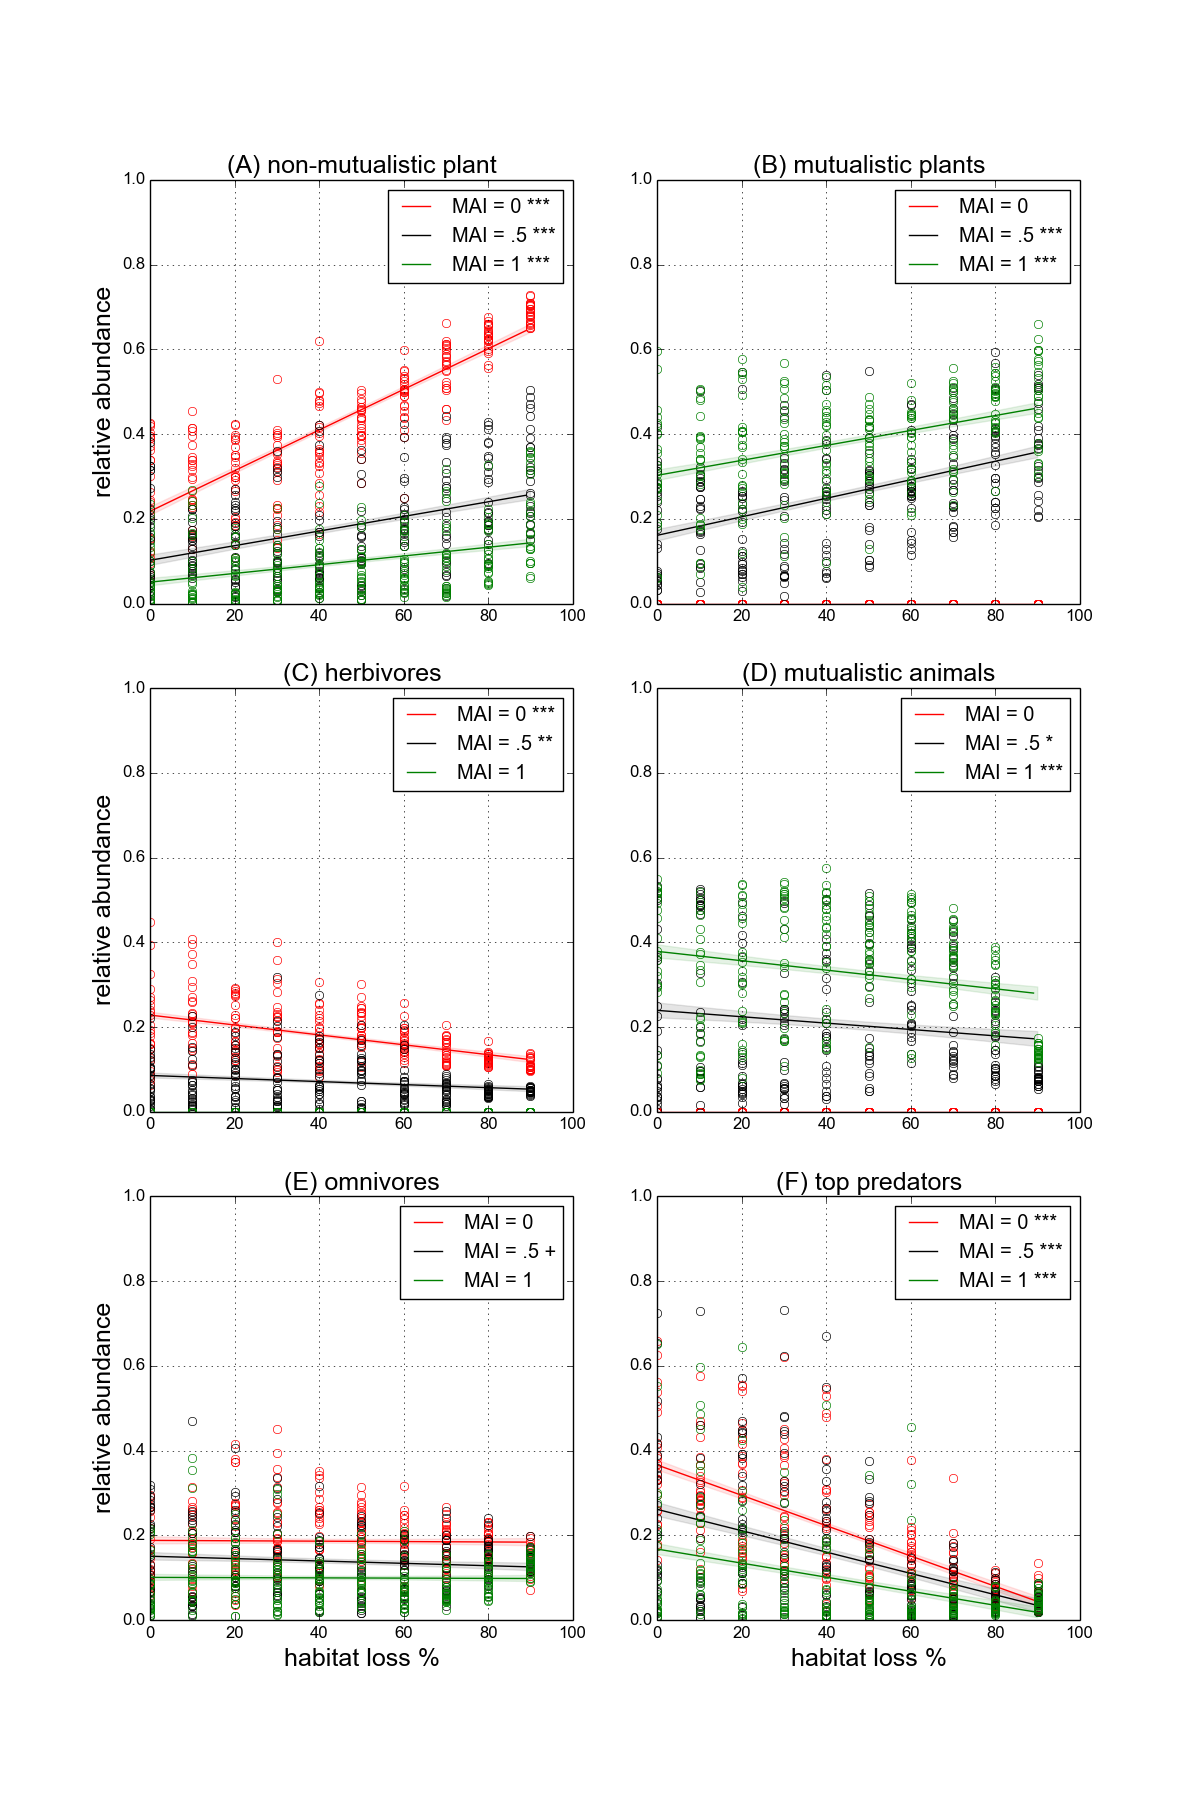
\includegraphics[width=\textwidth]{{{figures/bivariate_v_HL/lm_fg_relative_abundance_hl_random_3mai}}}
	\caption{\textbf{Relative abundance by FG}. Random}
	\label{fig:biv_HL_proportion_by_fg_random}
\end{figure}

\begin{figure}
	\centering	
	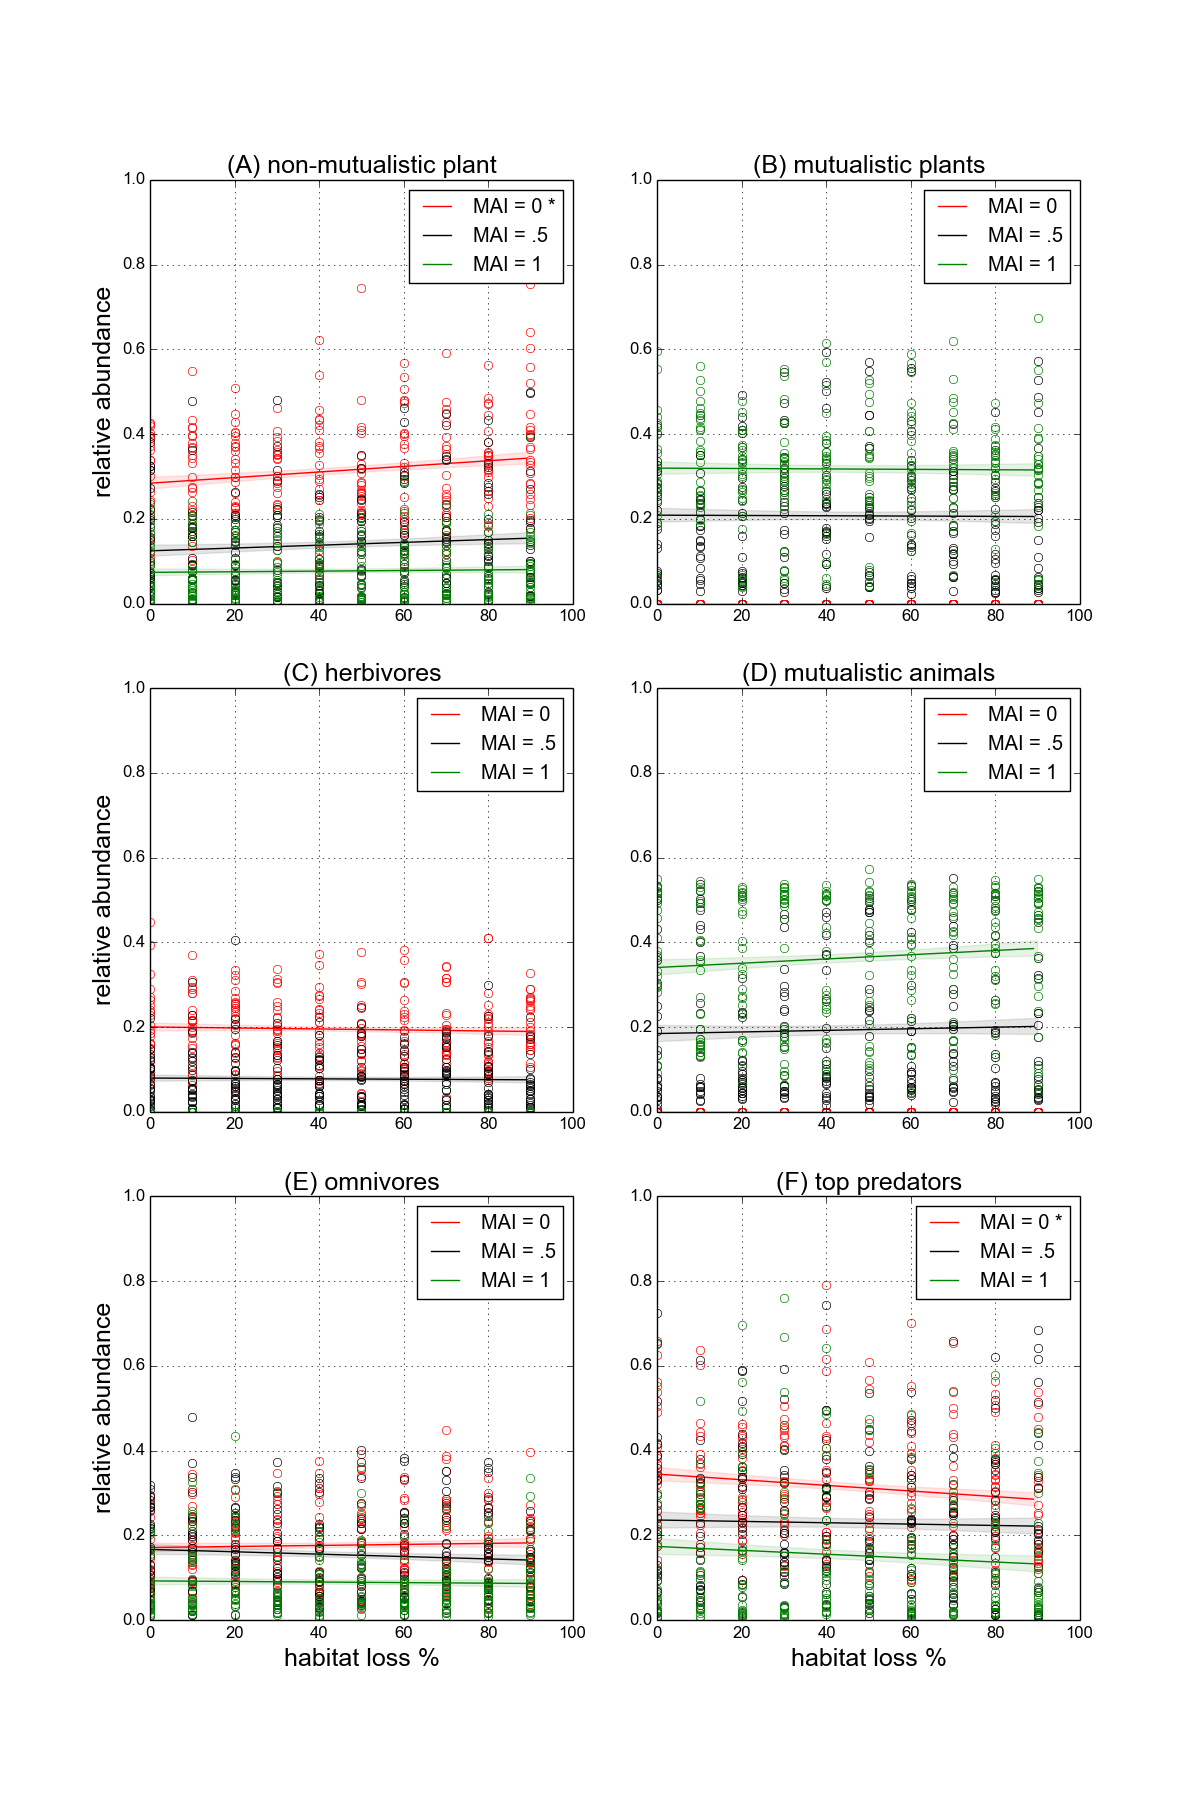
\includegraphics[width=\textwidth]{{{figures/bivariate_v_HL/lm_fg_relative_abundance_hl_contiguous_3mai}}}
	\caption{\textbf{Relative abundance by FG}. Contiguous}
	\label{fig:biv_HL_proportion_by_fg_contiguous}
\end{figure}

\begin{figure}
	\centering	
	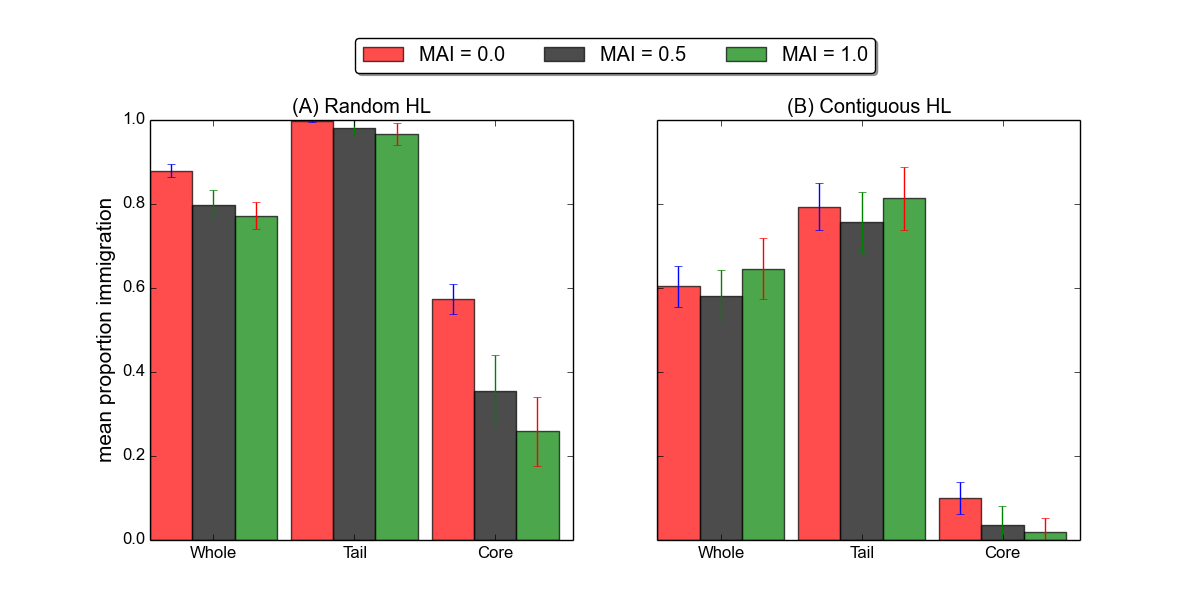
\includegraphics[width=\textwidth]{{{figures/bivariate_v_HL/dependence_IR_core_tail}}}
	\caption{\textbf{Dependence on immigration} at HL$=90\%$, split into tail, core and whole community.}
	\label{fig:biv_HL_tail_core}
\end{figure}


Why do mutualistic communities display more extinctions? - less even..
Why do mutualistic communities display fewer changes in evenness?

\section{Bivariate analysis: fixed HL}
\label{sec:biv_fixHL}

There are certain features of the summary results from section \ref{sec:init_res} that make it desirable to study communities along an IR gradient at fixed HL. In particular the observation that mutualistic communities do not change total abundance with IR is interesting. We are also interested in why interaction strengths change in response to IR, and why total abundance increases at low IR for antagonistic communities.

We may also be interested in the fact that reducing the IR does not necessarily reduce the dependence in immigration in a linear way - this is more subtle than we had previously imagined. It does reduce dependence until very low IR, when dependence suddenly increases again -perhaps due to the fact that there are too few individuals in the landscape to interact? Or perhaps because at these very low IRs a few species dominate, the majority of species just depend on immigrations.

Plots to produce:
\begin{itemize}
	\item Relative abundance by FG
	\item Possibly: RADs -> show that plants dominate, causing increase in abundance
	\item Interaction strength distributions for shifting IR - probably conclude that this is the same feature is variability - metrics tends to infinity at low abundance
\end{itemize}

\begin{figure}
	\centering	
	\includegraphics[width=\textwidth]{{{figures/bivariate_v_IR/example_RADS_mai0_random}}}
	\caption{\textbf{Example RADs} MAI$=0.0$ Random HL.}
	\label{fig:biv_IR_rads_mai0_random}
\end{figure}

\begin{figure}
	\centering	
	\includegraphics[width=\textwidth]{{{figures/bivariate_v_IR/example_RADS_mai1_random}}}
	\caption{\textbf{Example RADs} MAI$=1.0$ Random HL.}
	\label{fig:biv_IR_rads_mai1_random}
\end{figure}

\begin{figure}
	\centering	
	\includegraphics[width=\textwidth]{{{figures/bivariate_v_IR/example_RADS_mai1_contiguous}}}
	\caption{\textbf{Example RADs} MAI$=0.0$ Contiguous HL.}
	\label{fig:biv_IR_rads_mai0_contiguous}
\end{figure}
\begin{figure}
	\centering	
	\includegraphics[width=\textwidth]{{{figures/bivariate_v_IR/example_RADS_mai1_contiguous}}}
	\caption{\textbf{Example RADs} MAI$=1.0$ Contiguous HL.}
	\label{fig:biv_IR_rads_mai1_contiguous}
\end{figure}

\section{Alternative definition of extinction}
\label{sec:extinction}

As stated we will investigate alternative definitions of extinction. These are the possible definitions:
\begin{itemize}
	\item Species that do no have any natural births (during a time period) i.e. only immigration, if any
	\item Species that do not interact with other species during a time period
	\item Species that are below a certain threshold (relative) abundance
\end{itemize}

We suspect that these different metrics will given similar results. Here we plot heatmaps based on the above three definitions.

\section{Discussion}
\label{sec:vir_discussion}

Are species `in the tail' interacting at all?

Random HL appears to be beneficial to low abundance species, in that they are not driven to extinction by predation/competition. However this benefit is only realised in the presence of immigration. As we saw in chapter \ref{chap:}, without immigration these species would be driven to extinction.

\section{Conclusion}
\label{sec:vir_conclusion}

%\newpage
%\section{Exploration of parameter space: habitat loss and immigration}
%\label{sec:heatmaps}
%
%\begin{figure}
%	%\centering	
%	\hspace{-2.5cm}
%	\includegraphics[width=1.3\linewidth]{"./chapters/chapter04/figures/init_proportions"}
%	\caption{Mean number of species belonging to each functional group for the three MAI ratios in consideration ($0.0,0.5,1.0$). The results are averaged over one thousand simulations with the given MAI ratio, selected from the total ensemble of simulations that were run for this chapter (and used to generate e.g. fig \ref{fig:summary_heatmaps_imvshl}). The species numbers depicted are independent of all simulation parameters, other than those that define the interaction network. That is the average number of species in each function group depends on the niche model parameters (connection and number of species ), the MAI ratio, and the trophic constraints that we impose. }
%	\label{fig:initial_proportions}
%\end{figure}
%
%
%% In order to do what exactly...?
%Motivated by the above we explore a two dimensional slice of parameter space. The immigration rate (IR) and the level of habitat destruction (HL) are varied and one hundred repeat simulations are conducted at each pair value. Therefore were are able to estimate how the simulated communities are expected to behave across this region of parameter space, by averaging over the repeats. These simulation are run for three different MAI ratios: 0.0, 0.5 and 1.0. As in previous simulations each repeat uses a different interaction network topology, generated with the procedure described in section \ref{sec:whereis}.  All other parameters are held constant at their default values (table \ref{tab:wehereis}), including the number of iterations which remains at 5000. 
%
%In order to speed up the simulations certain metrics used in the previous analysis (chapter \ref{ch:whereis}) are not calculated. Particulary the spatial stability metrics are computationally expensive. Only two pieces of information are saved as output from these simulations: the underlying network structure and the abundance time-series for each species. The abundance time-series is simply a record of the abundance of each species at every simulation iteration. (What do we calculate from these and why..) By limiting the simulation output the scope for analysis is restricted but the parameter space can be explored in more detail (higher resolution, greater number of repeats)\footnote{The changes to the model output reduced run times by up to a factor of 10. This required changes in how the interaction network is represented and therefore previously used network metrics could not be calculated. However it would be easy to modify the code to save some information on interaction frequencies and spatial states, which could be used in later analysis. This has not been done yet -ON THE WAY.}. This `first pass' scan of the parameter space allows us to construct a general picture of how the model behaves in this region. It may also be used to identify subsets of the  region of parameter space on which to focus further computational effort for e.g. spatial analysis.
%
%The entire range of habitat destruction is explored from pristine landscape ($0\% HL$) to near total destruction ($90\%HL$) in steps of $10\%$. In the current chapter all habitat is destroyed using the contiguous algorithm since it was decided that this is more realistic (see discussion in section \ref{sec:whereis}). Ranges for the IR were chosen based on previous simulations. Since $IR=0.005$ is sufficiently high to prevent any extinctions, this was taken as the maximum of the range. Simulations using $IR=0$ have already determined that this leads to community collapse, therefore these were not repeated. A value of $IR=0.0001$ was heuristically selected as the lower bound, at which some non-zero extinction is expected in pristine habitat for all MAI ratios\footnote{Dani thinks we should maybe look at lower IR values.}.
%
%The choice of MAI ratios allows us to compare purely antagonistic ($MAI=0.0$), mixed ($MAI=0.5$) and purely mutualistic ($MAI=1.0$) communities. Figure \ref{fig:initial_proportions} shows the expected fraction of species belonging to each of the six functional groups in the interaction networks for these communities. The constraints we place upon the niche model are that at least $25\%$, $25\%$ and $5\%$ belong to the first, second and fourth trophic levels respectively. In particular it is known that the unconstrained niche model struggles to generate realistic number of species in the second trophic level [REF]. The figure shows that the interaction networks meet these constraints and that, as expected, the largest number of species is found in the third trophic level\footnote{Perhaps these constraints should be changed in future simulations - discuss with Daniel. - he thinks OK. Suggests look at RADS with colouring by TL. REQUIRES LOOKING AT SINGLE NETWORK.} i.e. the functional group labelled \emph{omnivores}. Antagonistic communities are missing the two mutualist functional groups from the first two trophic levels, whereas the mixed communities have a roughly $50:50$ split between mutualists and non-mutualists as expected (this split is not exact because it is links that are switched no species). Importantly although the purely mutualistic communities contain no herbivores (as all their links to plants have been switched), they do contain non-mutualist plants. These plants are those that share no interactions with the first trophic level\footnote{Is this realistic - Daniel? - RESTSAE QUESTION: REAlISTIC THAT PLANTS ARE NOT EATEN BY FIRST TROPHIC LEVEL..}, therefore the link replacement procedure does not give them any mutualist partners. These plants remain wind dispersed and are predated upon by animals from trophic levels three and four\footnote{Should there be a constraint that top predators do not consume plants? Not in original niche model. (Dani says no. Re-run. Does it make a difference?}.   
%
%%%%%%%%%%%%%%%%%%%%%%%%%%%%%%%%%%%%%%%%%%%%%%%%%%%%%%%%%%%%%%%%%%%%%%%%%%%%%%%%%%%%%%%%%%%%%%%%%%%%%%%
%%% Archetypal rotated figure page:
%%% STILL BEING A PAIN IN THE ARSE - NEEDS WORKING ON!
%%\newpage
%\clearpage
%%\afterpage{%
%\thispagestyle{empty}
%\begin{sidewaysfigure}
%
%		\centering      
%		\hspace{-3cm}
%
%        \includegraphics[width=\linewidth]{"./chapters/chapter04/figures/sum_maps"}
%        \caption{\textbf{Summary heat maps:} Each heat map shows the value of a certain response metric across a 2-dimensional slice of parameter space. The parameters varied are immigration rate $IR$ (y-axis) and percentage habitat destruction $HL$ (x-axis). Each row of plots corresponds to a different MAI ratio as labelled. To construct the heatmaps one hundred repeat simulations were run for each combination of parameter values, with each simulation using a different underlying network. The mean value of the response metrics is taken over the hundred repeats. Therefore each pixel shows an estimate of the expectation value of the metric at those parameter values. The left column shows the expected number of species that are extinct at the end of a simulation; the central column shows the expected biomass (total number of individuals) at the end of a simulation; and the right column shows the expected temporal variablity (coefficient of variaiton of total biomass) of the dynamics during the final thousand iterations of a simulation. The latter is used as a proxy for stability (see text).}\label{fig:summary_heatmaps_imvshl}
%        %% Note: this figure generated by Documents/IM_vs_HL_heatmap/plot_sum_maps.py
%\end{sidewaysfigure}
%\clearpage
%%}
%%%%%%%%%%%%%%%%%%%%%%%%%%%%%%%%%%%%%%%%%%%%%%%%%%%%%%%%%%%%%%%%%%%%%%%%%%%%%%%%%%%%%%%%%%%%%%%%%%%%%%%
%
%\subsection{Summary heat-maps}
%\label{sec:sum_heat_maps}
%
%The results of these simulations can be concisely represented as heat maps over the region of parameter space explored. Figure \ref{fig:summary_heatmaps_imvshl} shows how the expected value of three summary metrics varies across this space: the number of extinct species, community biomass (total number of individuals) and temporal variability in community biomass. The response of each of these metrics is discussed individually below. The latter is used as a proxy for stability and is measured by the coefficient of variation (CoV) of the community biomass about its mean during the final thousand iterations of a simulation. (later..) This metric is often used to assess dynamic stability, but should not be confused with rigorous mathematical metrics relating to the stability of the equilibrium state of the system [REF]. It should be noted that the other two metrics, and all abundance measures in the following analysis, are calculated from a snapshot of the system state on the final iteration of a simulation. (Dani points out that average over replicates.., compare with averaged analysis, and discuss in context of steady state.) 
%
%\subsubsection*{Extinctions}
%
%No species extinctions are expected for sufficiently high levels of IR, across the whole range of HL values and for all MAI ratios. This results is visible in the left column of figure \ref{fig:summary_heatmaps_imvshl} and was already discussed in section \ref{sec:whereis}. It is found that reducing the IR leads to an increasing number of extinctions. At low IR extinctions are possible, even in pristine landscape. This fits the previous observation that zero IR always leads to community collapse.
%
%Increasing HL generally increases the number of expected extinctions. However nowhere in the parameter space do we see community collapse. In the most extreme case of low IR and high HL ($MAI=1.0,HL=90,IR=0.0001$) an average of close to thirty extinctions may be expected. Although this expected loss of half of the species is fairly catastrophic, it does not guarantee total collapse of the community. The trophic constraints imposed in the food-web generation procedure ensure that at least $25\%$ of species belong in the first (basal) trophic level (figure \ref{fig:initial_proportions}). In practice this very rarely (quantify) reaches above $30\%$. Therefore a loss of thirty species suggests that at least $40\%$ of the remaining species are non-basal\footnote{If all thirty species lost are non-basal we are left with $3/5$ basal species to $2/5$ non-basal. IN NATURE HIGHER TROPHIC LEVELS USUALLY MORE VULNERABLE [REF]. IS THIS THE CASE. OOO, COMMUNITY COLLAPSE.}. In other words, despite significant loss of species, there is some persistence in higher trophic levels. 
%
%For all three MAI ratios there exists an IR where the expected number of extinctions is zero in pristine landscape, but increases with HL. So although the immigration rescue effect prevents total community collapse, we do have a situation where HL can initiate species extinctions. The IR at which extinctions are initiated is increased by increasing the MAI ratio. This effect of MAI ratio on extinctions is general. On average we expect a greater number of extinctions for high MAI (1.0) than for low MAI ratio (0.0), all else being equal. At the lowest IR and with pristine habitat we may expect about one extinction with a MAI ratio of 0.0, compared to about ten extinctions with a MAI ratio of 1.0. This can possibly be explained by looking at the second column in figure \ref{fig:summary_heatmaps_imvshl}. On average a higher MAI ratio lead to a greater total number of individuals at the end of a simulation\footnote{Mechanism behind this? - From the Theoretical Ecology paper: "communities with larger MAI ratios hosted a larger number of individuals $(F(1273) = 98.69, p < 0.001)$ (Fig. 4). In spite of a decline in the abundance of non-mutualistic primary producers and herbivores with increasing MAI ratios (as expected due to a larger fraction of mutualistic species), the increase in mutualistic plants and animals overcompensated for this loss, causing an overall increase in abundance. This overcompensation was due to mutualistic plants becoming more abundant than non-mutualistic ones since mutualistic consumers do not consume as much resources from them and are, additionally, beneficial for their reproduction.}. This means that there are fewer empty landscape cells into which an individual may immigrate at random. This reduces the \emph{effective immigration rate} and so weakens the rescue effect. Any very rare species, only made viable by immigration, will be the ones hit by this and are likely to go extinct\footnote{To determine if this is what is happening need to look at total abundances?}. 
%
%\subsubsection*{Community biomass}
%%\label{sec:com_bio}
%There are strong trends in expected community biomass. Increasing HL has a negative effect on community biomass. This is intuitive and has been seen before. Also previously discussed (chapter \ref{ch:whereis}) is the result that, on average, communities with higher MAI ratio can support a greater biomass. However this effect is striking in these results, especially at low levels of HL. In a pristine habitat with an IR of 0.005, the expected number of individuals for a community with $MAI=0.0$ is around $20,000$, compared to around $50,000$ for a community with $MAI=1.0$. In fact, across the parameter space, purely mutualistic communities have around twice the biomass of purely antagonistic ones. Therefore in some sense mutualism appears to be `better' for the community. (Dani: although having more individuals means rescue effect less likely, and perhaps increase competition for space)  In section \ref{sec:whereis} we discuss whether it is better for the community as a whole, or only for those species that engage in mutualistic interactions.
%
%For antagonistic communities ($MAI=0.0$) the biomass is dependent on IR. Both very high and very low IRs support high biomass, whereas intermediate IRs support less (central panel, top row, figure \ref{fig:summary_heatmaps_imvshl}). The effect of high IR is intuitive - births due to high immigration supplement births due to reproduction in the local community. This supplementary effect is greater at higer IR. However the increase in biomass at very low IR is harder to explain. We know that at zero IR all non-plant species go extinct [REF CHPAT/SEC]. So we may expect that in the region of low IR non-plant species become increasingly rare\footnote{This can be checked later..}. In an antagonistic community this means a reduction in the number of herbivores and omnivores, which will benefit plant species. Therefore we may propose that the increase in the biomass at low IR is accounted for by an increased abundance of plants\footnote{This proposed mechanism may be working in reverse in the MAI=1.0 communities.}. This reasoning suggests that we should expect a difference in composition between the abundant antagonistic communities seen at low and high IR (see section \ref{whereis} - ABUNDANCE DISTS.).    
%
%Mutualism removes the dependence of community biomass on IR. Although the total biomass does not vary with IR for these communities ($MAI=0.5,1.0$) there may be changes in community composition. For example it is still reasonable to suspect that non-plant species become increasingly rare at low IR. However in a mutualistic community this has a different effect. It will benefit those plants that still have antagonistic interactions, but it will be detrimental to mutualist plants since they will be less likely to interact with a partner and therefore less likely to reproduce. So we may expect a shift in the relative abundances of the two functional groups of plants in favour of the antagonists at low IR (see section \ref{sec:rel_abun}).
%
%%% INCLUDE ELSEWHERE?? This is because the immigration mechanism provides a significant recovery effect.   It allows species that have gone locally extinct (from the simulation landscape) to recover by occupying empty cells. Therefore, for immigration values close to those used in the original simulations (chapter \ref{sec:where}), the average number of species that have gone extinct at the end of a simulation is close to zero\footnote{Since it is possible for a species to go extinct and to subsequently recover it may be sensible to use another definition of 'extinct'.}. This is true for all MAI ratios as shown by the left 
%
%\subsubsection*{Temporal variation}
%%\label{sec:temp_var}
% 
%In general increasing HL increases the temporal variablity of the dynamics. That is, communities are less stable in damaged landscapes. This result is only seen in the case of contiguous habitat destruction, as opposed to random destruction, and is discussed in more detail in section \ref{sec:wehreis} where it was shown to be associated with changes in the distribution of interaction strengths. Also communities are less stable at lower IR. This fits with previous results. It has been shown that communities are very stable and resistant to HL at high IR (section \ref{sec:whereis}). It has also been shown that they are unstable at zero IR, exhibiting community collapse (section \ref{sec:whereis}). This suggests that the model has a stable and an unstable regime, and that there must be a transition between the two when moving form high to low IR. The right-hand column of figure \ref{fig:summary_heatmaps_imvshl} shows a signature of this. Interestingly the loss of dynamic stability is greatest for antagonistic communities and weakest for purely mutualistic communities. This suggests that mutualism has a stabilising affect on community dynamics. It appears to confer better dynamic stability in the face of HL and changing IR (but there are also more extinction as discussed..).
%
%Another interesting feature of the CoV plots is that the trends described above appear to be broken at very low IR and high HL, where an increase in stability is visible. One potential mechanism is that this is an averaging effect. If some communities are totally collapsing in this region they would exhibit stable dominance of plant species, which would contribute positively to average community stability. However it may be that this effect is due to another mechanism.
%
%As mentioned previously the loss of dynamic stability is troubling since it calls into question the way that we calculate abundance metrics. Therefore the conclusions drawn in the following discussion may not be general and may not hold if the metrics were averaged over a number of iterations.(Dani: don't stress this here, put in limitations section.)
% 
% 
%\newpage
%\subsection{Example dynamics}
%\label{sec:example_dynamics}
%
%\begin{figure}[h!]
%	\centering	
%	%\hspace{-2.5cm}
%	\includegraphics[width=0.8\linewidth]{"./chapters/chapter04/figures/total_biomass_dynamics_hl_0_mai_0"}
%	\caption{Temporal dynamics of the total biomass of communities over the course of six simulations. Each panels shows the dynamics for three distinct simulations, each in a different colour. The left panels shows communities with a high immigration rate, and the right panel for a low immigration rate. In all cases there is no habitat destruction $HL=0$.}
%	\label{fig:total_biomass_dynamics}
%\end{figure}
%
%
%Figure \ref{fig:total_biomass_dynamics} illustrates the loss of stability in passing from a high to a low IR regime. This transition was proposed in section \ref{sec:temp_var}. The dynamics of three example antagonistic communities are depicted for each regime. These communities were selected at random from the one hundred repeat simulations at these parameter values. Antagonistic communities are shown because the increase in temporal variability is greater for these than for those with mutualism (see figure \ref{fig:summary_heatmaps_imvshl}). 
%
%In the high IR regime, shown in the left-hand panel of figure \ref{fig:total_biomass_dynamics}, we see that the total biomass of each community undergoes an initial transience followed by a period of relative stability. It appears that, during this second period, the system is undergoing stochastic fluctuations about its stable equilibrium\footnote{Test for this?}. In the low IR regime, shown in the right-hand panel, we see that the community biomass exhibits large scale fluctuations throughout the course of the simulations. It is not clear from inspection that the system is being perturbed about a stable equilibrium.\footnote{I would rephrase this. For example: there are different explanations for this patter: (i) Explanation 1, (ii) Explanation 2.} It may be that the reduction in IR increases the length of the initial transience, and that the communities illustrated are yet to reach steady-state after 5000 iterations. Or it may be that these communities reach their steady-state, but that the stochastic fluctuations are amplified because the equilibria are less stable\footnote{Further mathematical analysis to try and determine this? - Final chapter on model fitting?}. 
%
%\begin{figure}
%	\centering	
%	%\renewcommand{\thesubfigure}{}
%	%\setlength{\subfloatlabelskip}{0pt}
%	%\hspace{-2.5cm}
%	\subbottom[]{\includegraphics[width=0.8\linewidth]{"./chapters/chapter04/figures/trophic_dynamics_example_hl0_mai0"}}
%	%\caption{The mean initial number of species belogning to each functional gropup.}
%	%\label{fig:trophic_dynamics_example}
%	\subbottom[]{\includegraphics[width=0.8\linewidth]{"./chapters/chapter04/figures/trophic_dynamics_example2_hl0_mai0"}}
%	\caption{Dynamics from four individual simulation runs, with biomasses aggregated by trophic level. Each panel represents the dynamics of a single simulation run. In all cases the MAI ratio is $0.0$, and there is \textbf{no habitat destruction} ($HL=0$).  The coloured lines represent the temporal dynamics of the biomass of each trophic level, as indicated in the legends. Two immigration scenarios are presented. \textbf{Left column: high immigration. Right column: low immigration.}}
%	\label{fig:trophic_dynamics_example}
%	
%\end{figure}
%
%Figure \ref{fig:trophic_dynamics_example} shows example dynamics by trophic level of four antagonistic communities in the high and low IR regimes. The left-hand panels depict two communities in the high IR regime. Again the initial transience is followed by a period of relative stability, which is consistent across trophic levels. It is clear from these two plots that the positions of the system's equilibria and the size of the fluctuations about it vary between simulations.  
%
%The right-hand panel of figure \ref{fig:trophic_dynamics_example} depicts two communities in the high IR regime. It is clear from inspection that the mean and the variance of the biomasses varies between trophic level, and between simulation. The lower plot shows dynamics dominated by species from the first trophic level, with large scale but decreasing amplitude fluctuations in the second trophic level. The upper plot shows perhaps even less stable dynamics with increasing amplitude fluctuations in the first and fourth trophic levels, and very low abundances in the intermediate trophic levels. In both simulations there are several instances where the biomass of an entire trophic level comes close to zero. However, as figure \ref{fig:summary_heatmaps_imvshl} shows, we should only expect around one extinct species at the end of a simulation at this IR. It must be that that immigration is preventing stochastic extinctions here\footnote{At this IR we would expect on average four immigrations per iteration, if the landscape were empty.}, by providing some buffering to populations at the low end of their biomass fluctuations and by rescuing those species that do go extinct\footnote{It would be interesting to look at the breakdown of these trophic dynamics by species - e.g. how synchronous are the different species in the same trophic level with each other.}.
%
%The breakdown of dynamics by trophic level demonstrates that the timing of measurement will affect the calculation of relative abundance metrics, and not just that of the aggregate community biomass. If the fluctuation in trophic biomass were more synchronous between levels, the timing of the measurement would be less significant. However the figure shows that even the ordering of trophic levels by abundance is dependent on time\footnote{This is beginning to look make the results seem invalid.}. Therefore further analysis should attempt to remove this time dependence by averaging biomasses over a number of iterations. The plots suggest that the increase in community biomass at low IR (discussed in section \ref{sec:com_bio}) may be a genuine effect. However it is hard to determine the contribution of the increased fluctuations without averaging the abundances over time.
%
%(There may be other points in parameter space where it would be informative to plot the dynamics...e.g. high mutualism region, temporally stable)
%(Could plot biomass dynamics, averaged over replicates?)
%
%\newpage
%\subsection{Relative abundances and abundance distributions}
%\label{sec:rel_abun}
%
%Contextualise - begin this section with the points made above that suggest useful to look at RADS.
%
%Figure \ref{fig:rel_abun_tl_mai_01} shows the mean relative abundance of each trophic level for antagonistic and mutualistic communities, across the parameter space.  For purely antagonistic communities the proportion of individuals in each trophic level varies strongly with IR and weakly with HL. At low IR antagonistic communities become dominated by plant species. This is in agreement with the mechanism proposed in section \ref{sec:com_bio}, whereby plants benefit from a scarcity of animal consumers at low IR. At high IR the distribution of biomass is much more even across trophic levels. In this region of parameter space the biomass of trophic levels one and four are roughly equal at around $30\%$, with the remaining $40\%$ of the biomass split fairly evenly between trophic levels two and three. This biomass distribution is not necessarily unrealistic for a community in nature, however it does not conform to the classic \emph{biomass pyramid} (see discussion in section \ref{sec:whereis}). In fact the distribution at low IR is much closer to the standard pyramid.
%
%Mutualistic communities (MAI=1.0) show much less variation in their trophic composition across the parameter space. The first two trophic levels are most abundant, with slightly more biomass in the first trophic level than the second. The third and the fourth trophic levels are much less abundant with around $20-30\%$ of the biomass split fairly evenly between them. This distribution is remarkably constant over the parameter space. Only at extreme levels of disturbance ($IR=0.0001, HL\geq 70 \%$) do the communities begin to be dominated by plants. 
%
%Figure \ref{fig:rel_abun_fg_mai_51} shows the mean relative abundance of each functional group for mutualistic communities with $MAI=0.5$ and $MAI=1.0$. As expected purely mutualistic communities are dominated by functional groups two and four (mutualistic producer and animals) across the whole region of parameter space. Functional groups five and six do relatively better at high IR and low HL. Whereas at low IR and high HL the relative abundance functional group 1 increases significantly. This is an indication of the shift in favour of antagonists, suggested in section \ref{sec:com_bio}, due to the low biomass making it hard for mutualists to reproduce and less likely that plants will be eaten. The same patterns are seen in the case of $MAI=0.5$, however the trends appear stronger since the relative abundances are less robust to changes in IR and HL.     
%
%
%
%\begin{figure}[h!]
%	\centering	
%	%\hspace{-2.5cm}
%	%\renewcommand{\thesubfigure}{}
%	%\setlength{\subfloatlabelskip}{0pt}
%	\subbottom[$MAI = 0.0$]{\includegraphics[width=0.8\linewidth]{"./chapters/chapter04/figures/rel_abun_tl_mai_0"}}
%	\subbottom[$MAI = 1.0$]{\includegraphics[width=0.8\linewidth]{"./chapters/chapter04/figures/rel_abun_tl_mai_1"}}
%	\caption{The relative abundance of species belonging to each of the four trophic levels. Above: MAI = 0.0. Below: MAI = 1.0. Each pixel on the heat maps corresponds to an average over one hundred repeat simulations at those parameter values. The abundances are measured at the end of each simualtion.}
%	\label{fig:rel_abun_tl_mai_01}
%\end{figure}
%
%
%\begin{figure}[h!]
%	\centering	
%	%\hspace{-2.5cm}
%	%\renewcommand{\thesubfigure}{}
%	%\setlength{\subfloatlabelskip}{0pt}
%	\subbottom[$MAI = 0.5$]{\includegraphics[width=0.9\linewidth]{"./chapters/chapter04/figures/rel_abun_fg_mai_5"}}
%	\subbottom[$MAI = 1.0$]{\includegraphics[width=0.9\linewidth]{"./chapters/chapter04/figures/rel_abun_fg_mai_1"}}
%	\caption{The relative abundance of species belonging to each of the six functional groups. Above: MAI = 0.5. Below: MAI = 1.0. Each pixel on the heat maps corresponds to an average over one hundred repeat simulations at those parameter values. The abundances are measured at the end of each simulation.}
%	\label{fig:rel_abun_fg_mai_51}
%\end{figure}
%
%\subsection{Rank abundance distributions}
%\label{sec:rads}
%
%These results, as with the other should be recalculated using averaged metrics.
%
%Figure \ref{fig:mean_rads} shows the mean rank abundance distributions for a range of IR and HL values. Communities with all three MAI ratios are shown in different colours. Across the parameter space mutualistic communities (blue) have less even distributions than antagonistic communities. This difference is more pronounced at low IR and high HL. 
%
%An interesting feature of the RADs is that some of them display an apparent discontinuity in the distribution. This is perhaps most pronounced in the bottom left panel of figure \ref{fig:mean_rads} ($IM=0.0001, HL=0, MAI=1.0$). A sigmoidal shape is a feature of log-normal abundance distributions and is often observed in natural communities [REF]. However this extreme case does not appear to fit. What is driving this distribution?  The `flat' section of low abundance species could be those species whose presence is sustained only by continuous immigration and which are therefore present in roughly equal abundances?   
%
%
%
%\clearpage
%\afterpage{%
%%\thispagestyle{empty}
%\begin{sidewaysfigure}
%
%		\centering      
%		\hspace{-3cm}
%
%        \includegraphics[width=0.9\linewidth]{"./chapters/chapter04/figures/single_rads"}
%        \caption{\textbf{Rank abundance distributions} for individual simulation runs, for nine different pair values of immigration rate and habitat destruction. Each dsitribution is for a single community at the end of an individual simulation run. The different colours correspond to different MAI ratios: red = 0.0; green = 0.5; blue = 1.0. And the different symbols correspond to different trophic levels: circle = 0; upwards triangle = 1; sqaure = 2; downwards traingle = 3.}
%        \label{fig:single_run_rads}
%        %% Note: this figure generated by Documents/IM_vs_HL_heatmap/plot_sum_maps.py
%\end{sidewaysfigure}
%}
%
%%\clearpage
%\afterpage{%
%\thispagestyle{empty}
%\begin{sidewaysfigure}
%
%		\centering      
%		\hspace{-3cm}
%
%        \includegraphics[width=0.9\linewidth]{"./chapters/chapter04/figures/mean_rads"}
%        \caption{\textbf{Average rank abundance distributions} over one hundred simulation runs, for nine different pair values of immigration rate and habitat destruction. Each dsitribution is calculated using the mean relative abundance of the ranked species, averaged over the final abundances of one hundred repeat simulations. The different colours correspond to different MAI ratios: red = 0.0; green = 0.5; blue = 1.0.}
%        \label{fig:mean_rads}
%        %% Note: this figure generated by Documents/IM_vs_HL_heatmap/plot_sum_maps.py
%\end{sidewaysfigure}
%}
%
%
%\section{Points for discussion (Rough Notes)}
%
%A comparison of the relative merits of being a mutualist versus a non-mutualist is worthwhile. Importantly it must be remembered that mutualistic interactions are also trophic interactions. In our case, energy is transferred from producer to animal. In nature for example the bee receives energy from the nectar, but also carries pollen to fertilise other flowers.  So there is some loss/detriment to the producer as well as the benefit of reproduction (These mechanisms are in place in the model through the bioenergetic parameters. Traditionally, simulating mutualistic communities has failed because the simulations ended in an 'orgy of mutual benefaction'). It is an interesting strategy from an evolutionary perspective...discuss this (with relation to link switching)?
%
%
%In the model species become mutualistic by having at least one of their links, in the antagonistic interaction network, switched for a mutualistic link. Table \ref{tab:parameters} shows the default parameter values used for most simulations. Lets consider the potential benefit of switching a single herbivorous link for a mutualistic link, for either party. If the plant is a non-mutualist it must impart 20\% of its energy to the offspring when reproducing (this happens with a probability of 0.01 on each iteration). It is also subject to lose 70\% when it is encountered by this herbivour. If it were to switch this herbviourous link for a mutualistic link it would only lose 25\% of its energy in the interaction, and it would pass on a seed that is almost guaranteed\footnote{Really? We could look at how many mutualistic interactions lead to a new individual. It would only not occur in very crowded situations.} to generate an offspring. Therefore the cost of reproducing is slightly increased for a mutualist, but the cost of interacting with an individual from the trophic level above is dramatically reduced. There is an additional benefit that the mutualistic reproduction can occur over a greater distance. The net gain loss of this change depends on the probability/rate of interactions. We should investigate this, however the results suggest that being a mutualist is of significant benefit to plants. (These mechanisms are in place in the model through the bioenergetic parameters. Traditionally, simulating mutualistic communities has failed because the simulations ended in an 'orgy of mutual benefaction')
%
%Question: in the above analysis are mutualistic plants are relatively more abundant than non-mutualistic ones, except in the case of high habitat loss or low immigration (when there are few enough mutualistic partners that interactions become infrequent?) 
%
%For animals there is no cost to carrying and spawning the seed of their mutualistic partners. The only change in the switching of mutalistic links is the amount of energy that they receive from the interaction. During a herbivourous interaction, the hebivore takes 70\% of the plant's energy, and assimilates it with an efficiency of 80\%. Therefore it obtains ~60\% of the plants energy. During a mutualistic interaction the animal-mutualist takes and assimilates 25\% of the plants energy. Therefore on an interaction by interaction basis there is a negative trade off for an animal in switching its link to mutualistic. However there may be an emergent benefit in that this type of interaction is much better for plants, therefore increasing the plant biomass and therefore indirectly benefiting animal (mutualists and non-mutualists?) due to the increased frequency of interactions (density of plants).       
%
%
%%% IMPORTANT POINTS:
%%\begin{itemize}
%%	\item Do mutualistic plants only reproduce mutualistically? (almost certain yes)
%%	\item Does MATINGRESOURCE apply to mutualistic interactions?
%%	\item Why are top predators able to eat plants?!! Does omnivory trade off apply?? - too many individuals belong to TL3 in general.
%%\end{itemize}
%
%
%Mutualism in general stabilises dynamics, and leads to communities with more realistic biomass pyramids - i.e. dominated by the first two trophic levels, with fewer individuals in TL2/3. 
%
%It could be argued that the RADS are realistic, and the some immigration is a requirement to prevent stochastic extinction of the very rare species, which are found in nature. This begs the question as to what mechanism prevents their extinction in nature? And are they the most vulnerable to extinction?  
%
%\section{Habitat loss with low immigration}
%
%\section{Questions for Alan or Daniel}
%
%\begin{itemize}
%	\item Worried about general flow and structure of discussion. Feels like trying to present too much information all at once. How to not turn into a list of facts, where the relevance gets lost?
%
%	\item Since the dynamics do not necessary reach steady state should I re-do analysis with average over a time window? (We need a discussion section where the results are discussed in the context of current literature in the field, real-world communities, etc. Also, contextualizing (see a previous comment) is important so the reader does not feel like we include all these metrics because we can. For doing this it is always helpful to write down the main findings as bullet points and develop them; also, the limitations of the model should be presented here as well as the ways forward)
%	\item Can I use "we"??
%	\item Tense?
%	\item Figure 1.1 summary heatmaps: too much information in one figure? (feels that way from discussion).
%	\item OK to use plant, basal and producer interchangeably?
%
%	\item The ability of the top predator to survive almost entirely on plant matter is troubling.
%	
%	\item Is it in fact OK to use biomass and number of individuals interchangeably? 	(We need a discussion section where the results are discussed in the context of current literature in the field, real-world communities, etc. Also, contextualizing (see a previous comment) is important so the reader does not feel like we include all these metrics because we can. For doing this it is always helpful to write down the main findings as bullet points and develop them; also, the limitations of the model should be presented here as well as the ways forward)
%	
%	%\item TODo: linear interactions? (should it be that freq/predabun should be linear in preyabun? Same gradient across species?) If so we should be able to fit a GLV, if not via Timme, then via repreated simulations and some numerical optimisation.
%	\item Theme for discussion seems to be developing: point out a feature of the results, explain what could be causing it (in the model), relate this to other results. (should add to this - comment on how this may relate to the real world??) (Agree. The discussion section to summarize and explain, contextualize the results is needed.)
%\end{itemize}
%
%RADS: Good. As the main changes are observed for different IR it is good to include plots of abundance vs rank with the lines representing different IRs. Also, it could be nice to see if they deviate from a classical lognormal or lognormal family type distribution (which is usually found in nature)
%
%Are the legends correct? The plots next to this note are similar. I think they have different IR, right?

